\section*{Step 3}

\begin{custombox}[label={box:Q3}]{Step 3}
	Generate outputs by setting \textbf{degree = 1}, \textbf{degree = 3}, \textbf{degree = 6}, \textbf{degree = 10}, in the \verb|PolynomialFeatures| function used in \verb|E3.ipynb| and analyze them as follows:
	\begin{enumerate}[label=(\alph*)]
		\item Review the \verb|augmented_data.csv| file generated in each case and document your observations.
		\item Create an overall qualitative summary based on a review and analysis of the Figures generated.
		\item Summarize and explain the variations in the metrics \textbf{across regression methods for a given degree} (ie. a given set of polynomial features). Cover both, train and test, metrics, and compare them.
		\item Summarize and explain the variations in the metrics \textbf{across degrees for a given regression method}. Cover both, train, and test metrics, and compare them.
		\item When \textbf{degree = 1} which method(s) result in acceptable regression models? Why?
		\item When \textbf{degree = 6} which method(s) result in acceptable regression models? Why?
		\item As the value of degree is increased to 10 which regression methods show the most impact? Why?
		\item Why do non-parametric methods like \verb|KNN| and \verb|Decision Tree| based methods generate good results even without feature engineering?
		\item What are the limitations of the non-parametric methods?
		\item  Given the results, should LinearRegression be used at all? Why, when? Justify your answer.
	\end{enumerate}
\end{custombox}

\begin{customboxnew}[label={box:Q3a}]{Question (a)}
	Review the \verb|augmented_data.csv| file generated in each case and document your observations.
\end{customboxnew}

The following observations are based on the content of the \verb|augmented_data.csv| files generated for different polynomial degrees:

\begin{itemize}
    \item \textbf{Degree = 1:}
    \begin{itemize}
        \item \textbf{File Content:} The \verb|augmented_data.csv| file contains only the original feature and the target variable \( y \). With degree = 1, no additional polynomial features are generated beyond the original feature.
        \item \textbf{Observation:} The file contains columns for the original feature(s) plus the target variable \( y \). There are no new features created.
    \end{itemize}
    
    \item \textbf{Degree = 3:}
    \begin{itemize}
        \item \textbf{File Content:} The file includes the original feature \( x_1 \) along with polynomial terms up to the third degree: \( 1 \), \( x_1 \), \( x_1^2 \), and \( x_1^3 \), plus the target variable \( y \).
        \item \textbf{Observation:} The file contains columns for the original feature, its squared term, its cubic term, and the target variable \( y \). There are four columns in total.
    \end{itemize}
    
    \item \textbf{Degree = 6:}
    \begin{itemize}
        \item \textbf{File Content:} This file contains the original feature \( x_1 \) and polynomial terms up to the sixth degree: \( 1 \), \( x_1 \), \( x_1^2 \), \( x_1^3 \), \( x_1^4 \), \( x_1^5 \), \( x_1^6 \), plus the target variable \( y \).
        \item \textbf{Observation:} The file includes the original feature, its polynomial terms up to the sixth degree, and the target variable \( y \). There are eight columns in total.
    \end{itemize}
    
    \item \textbf{Degree = 10:}
    \begin{itemize}
        \item \textbf{File Content:} For degree = 10, the file contains the original feature \( x_1 \) and polynomial terms up to the tenth degree: \( 1 \), \( x_1 \), \( x_1^2 \), \( x_1^3 \), \( x_1^4 \), \( x_1^5 \), \( x_1^6 \), \( x_1^7 \), \( x_1^8 \), \( x_1^9 \), \( x_1^{10} \), plus the target variable \( y \).
        \item \textbf{Observation:} The file has columns for the original feature and its polynomial terms up to the tenth degree, along with the target variable \( y \). There are twelve columns in total.
    \end{itemize}
\end{itemize}

\begin{figure}[H]
	\centering
	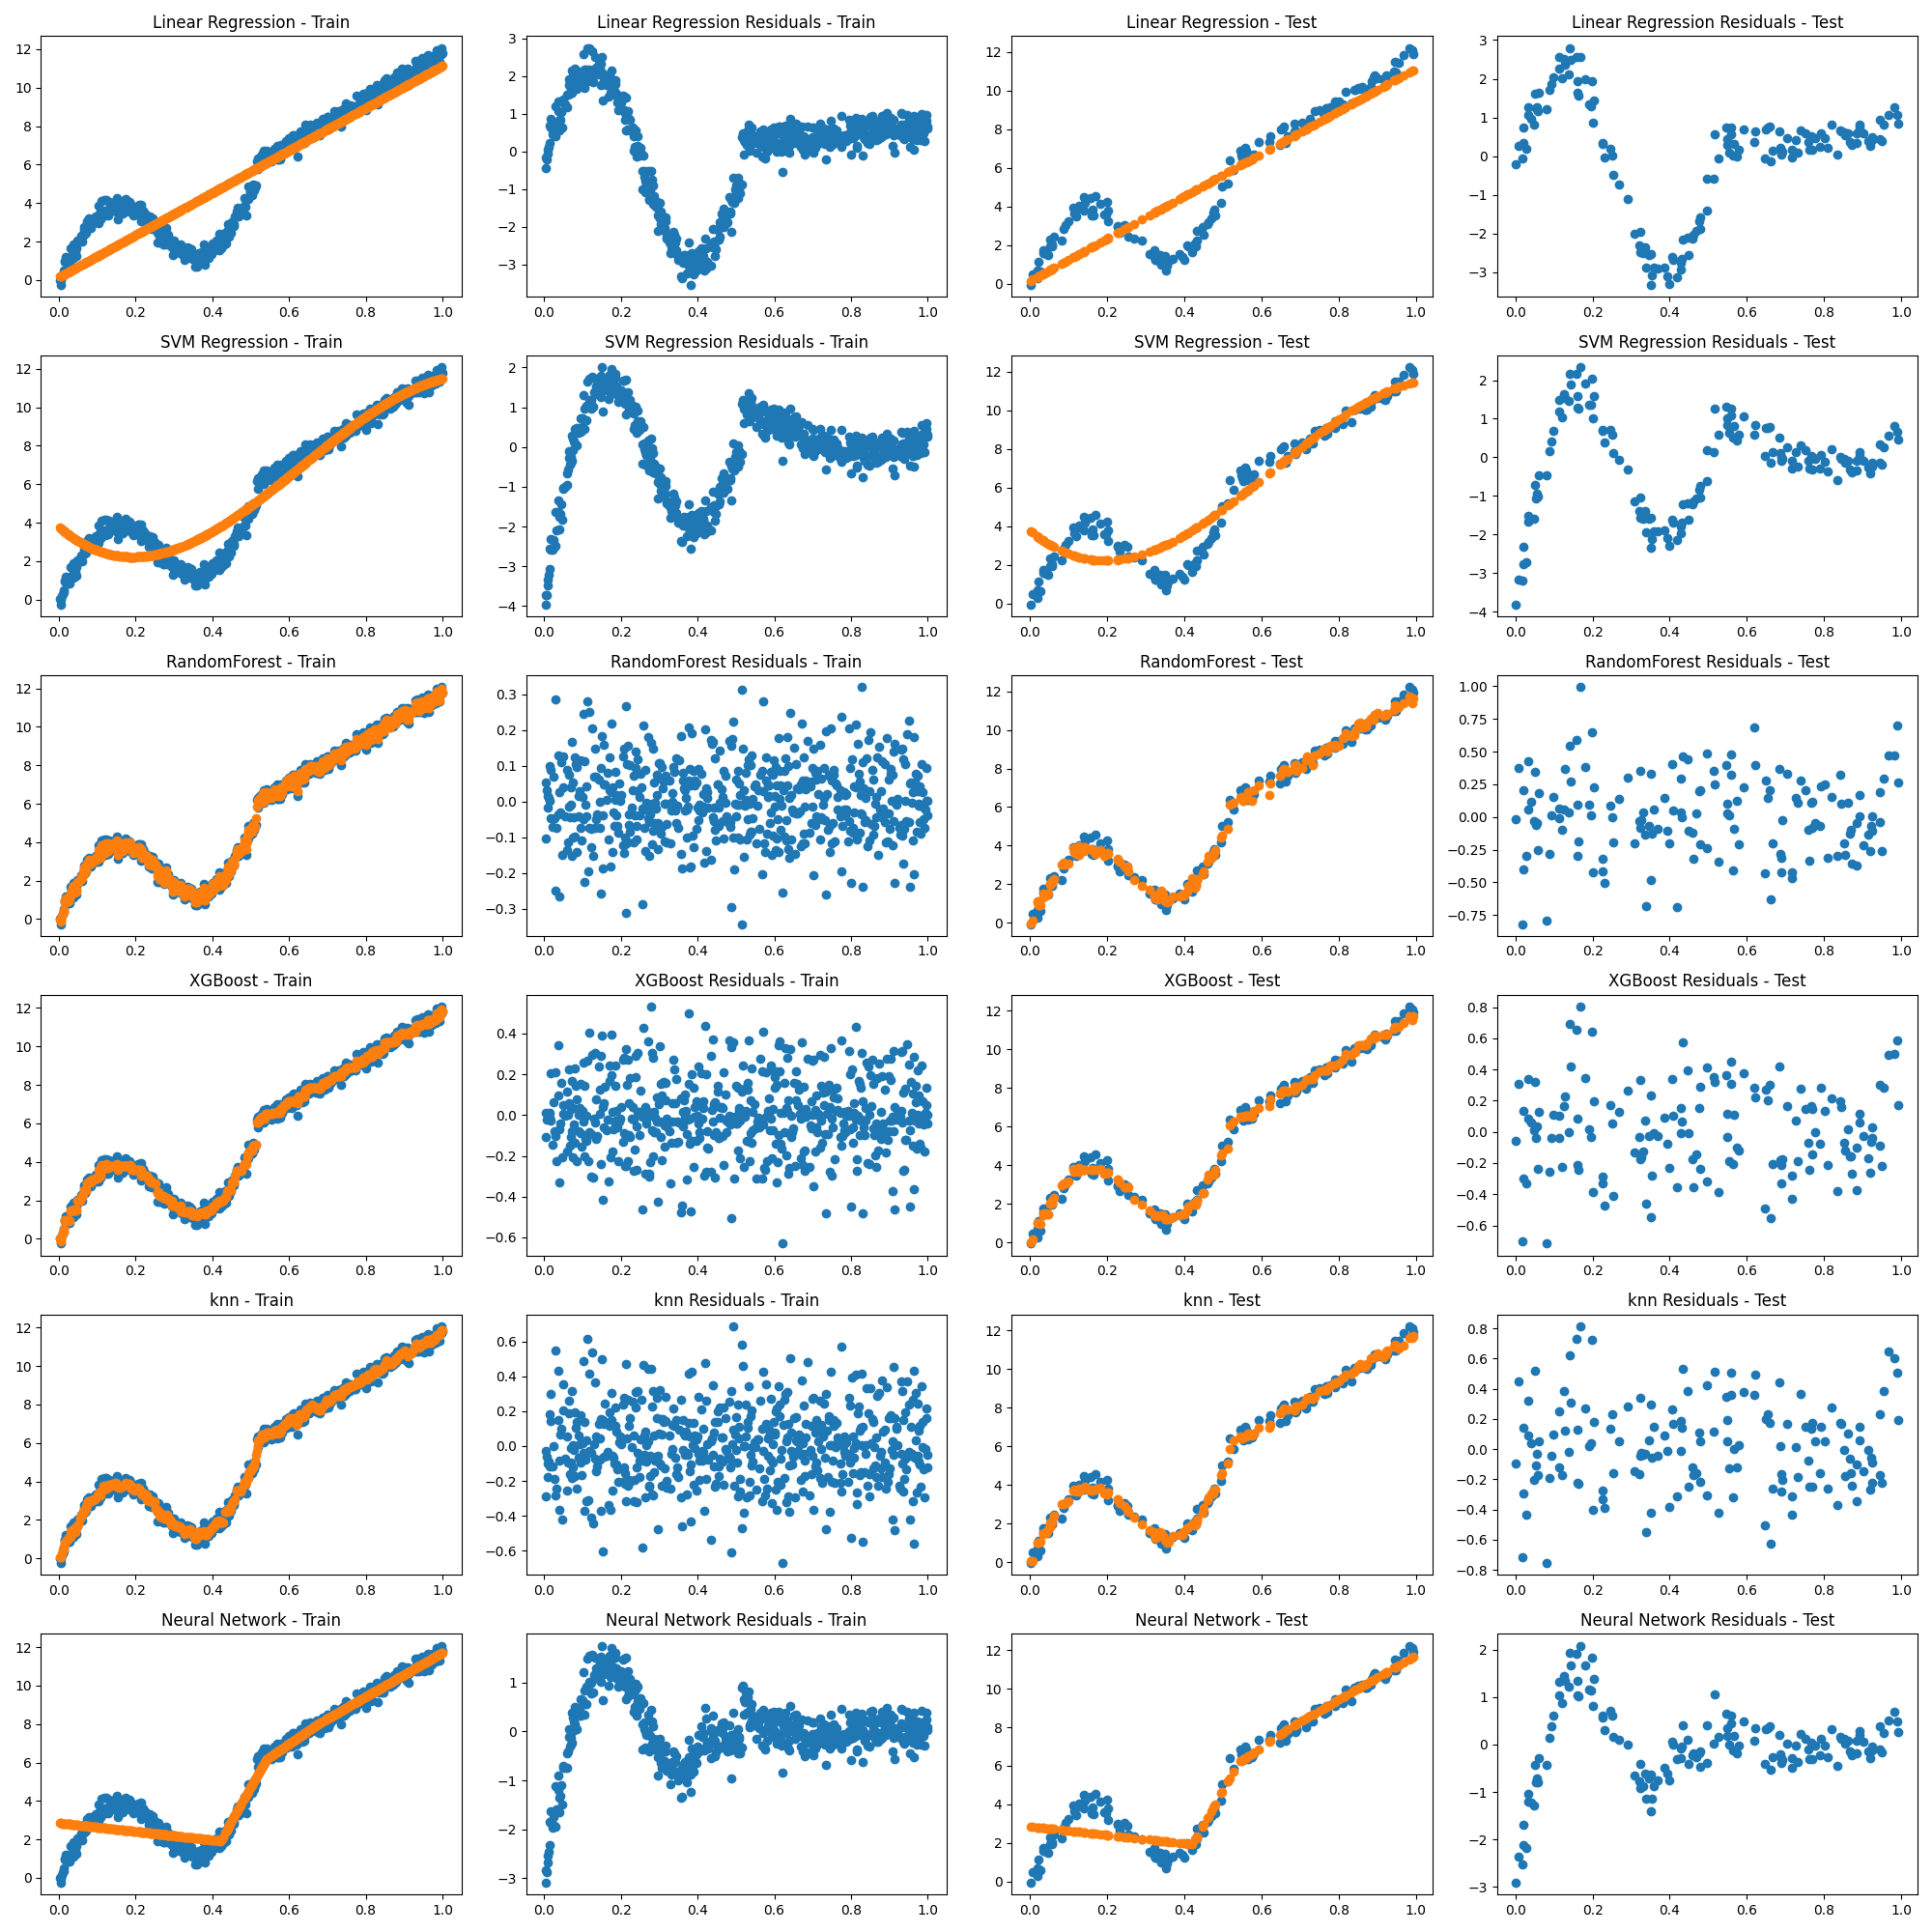
\includegraphics[width=0.8\linewidth]{./Images/E3-MLR3-1.png}
	\caption{Various Regression Models with degree = 1}
\end{figure}

When degree = $1$, the following observations can be made:

\begin{itemize}
    \item \textbf{Linear Regression:} The plot reveals significant underfitting, with the linear fit failing to capture the non-linear trends in the data.
    \item \textbf{SVM (Polynomial Kernel):} The SVM plot shows similar underfitting as Linear Regression, with the linear decision boundary not aligning well with the non-linear data distribution.
    \item \textbf{RandomForest:} The plot demonstrates better fit compared to linear models, with RandomForest capturing some non-linear patterns despite the linear feature expansion.
    \item \textbf{XGBoost:} XGBoost effectively models the non-linear relationships, as seen in the plot with predictions aligning more closely with the true data distribution.
    \item \textbf{K-Nearest Neighbors (KNN):} The KNN plot indicates a good fit to the non-linear data, showing accurate predictions based on proximity without needing polynomial features.
    \item \textbf{Neural Network:} The plot for the Neural Network shows a strong fit to the non-linear data, capturing complex patterns despite the linear feature input.
\end{itemize}

\begin{figure}[H]
	\centering
	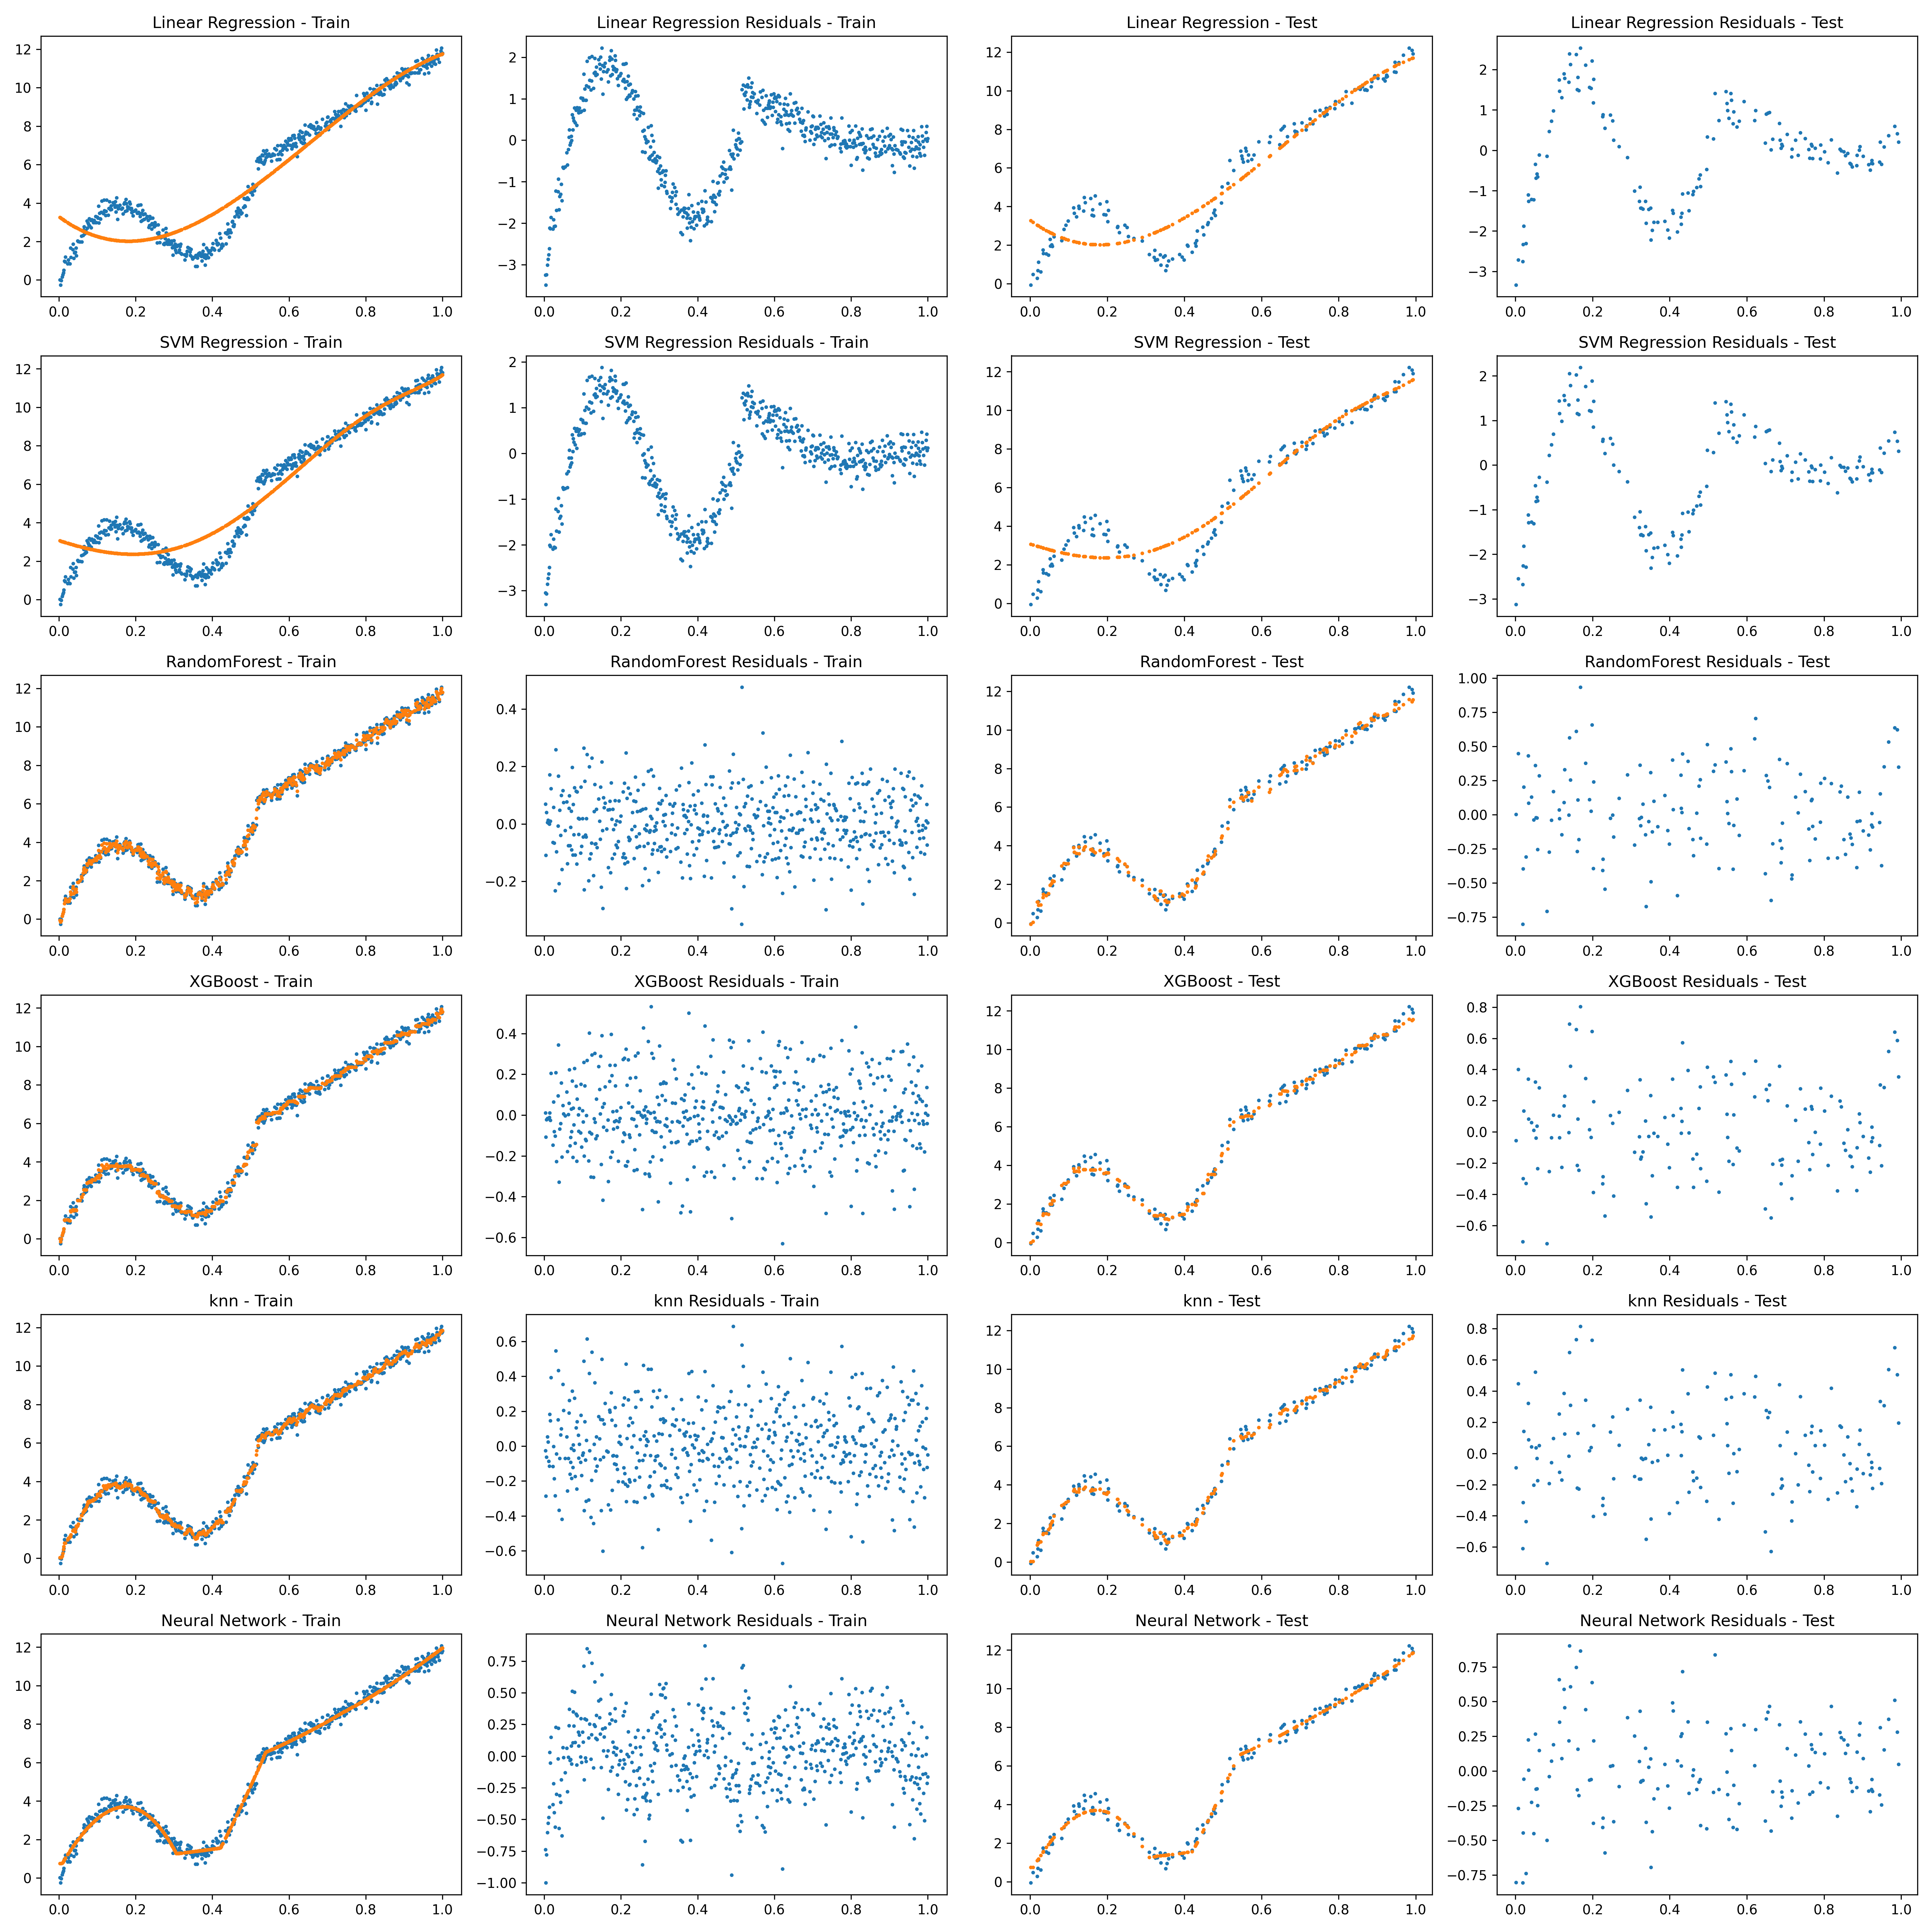
\includegraphics[width=0.8\linewidth]{./Images/E3-MLR3-3.png}
	\caption{Various Regression Models with degree = 3}
\end{figure}

\begin{itemize}
    \item \textbf{Linear Regression:} The plot shows improved fit over degree = 1 but still exhibits signs of underfitting, as the linear model struggles to capture the higher-order non-linear patterns.
    \item \textbf{SVM (Polynomial Kernel):} The linear SVM plot still underfits, with the decision boundary unable to fully align with the more complex, non-linear data distribution.
    \item \textbf{RandomForest:} The plot indicates a good fit, capturing more of the non-linear structure compared to degree = 1, thanks to its ability to model complex interactions.
    \item \textbf{XGBoost:} The XGBoost plot shows a strong fit to the non-linear data, effectively utilizing the higher-order polynomial features to model intricate patterns.
    \item \textbf{K-Nearest Neighbors (KNN):} The KNN plot reflects an excellent fit, with predictions closely following the non-linear trends in the data, demonstrating its strength with complex features.
    \item \textbf{Neural Network:} The Neural Network plot exhibits a very accurate fit, capturing complex non-linear relationships effectively with the expanded polynomial features.
\end{itemize}

\begin{figure}[H]
	\centering
	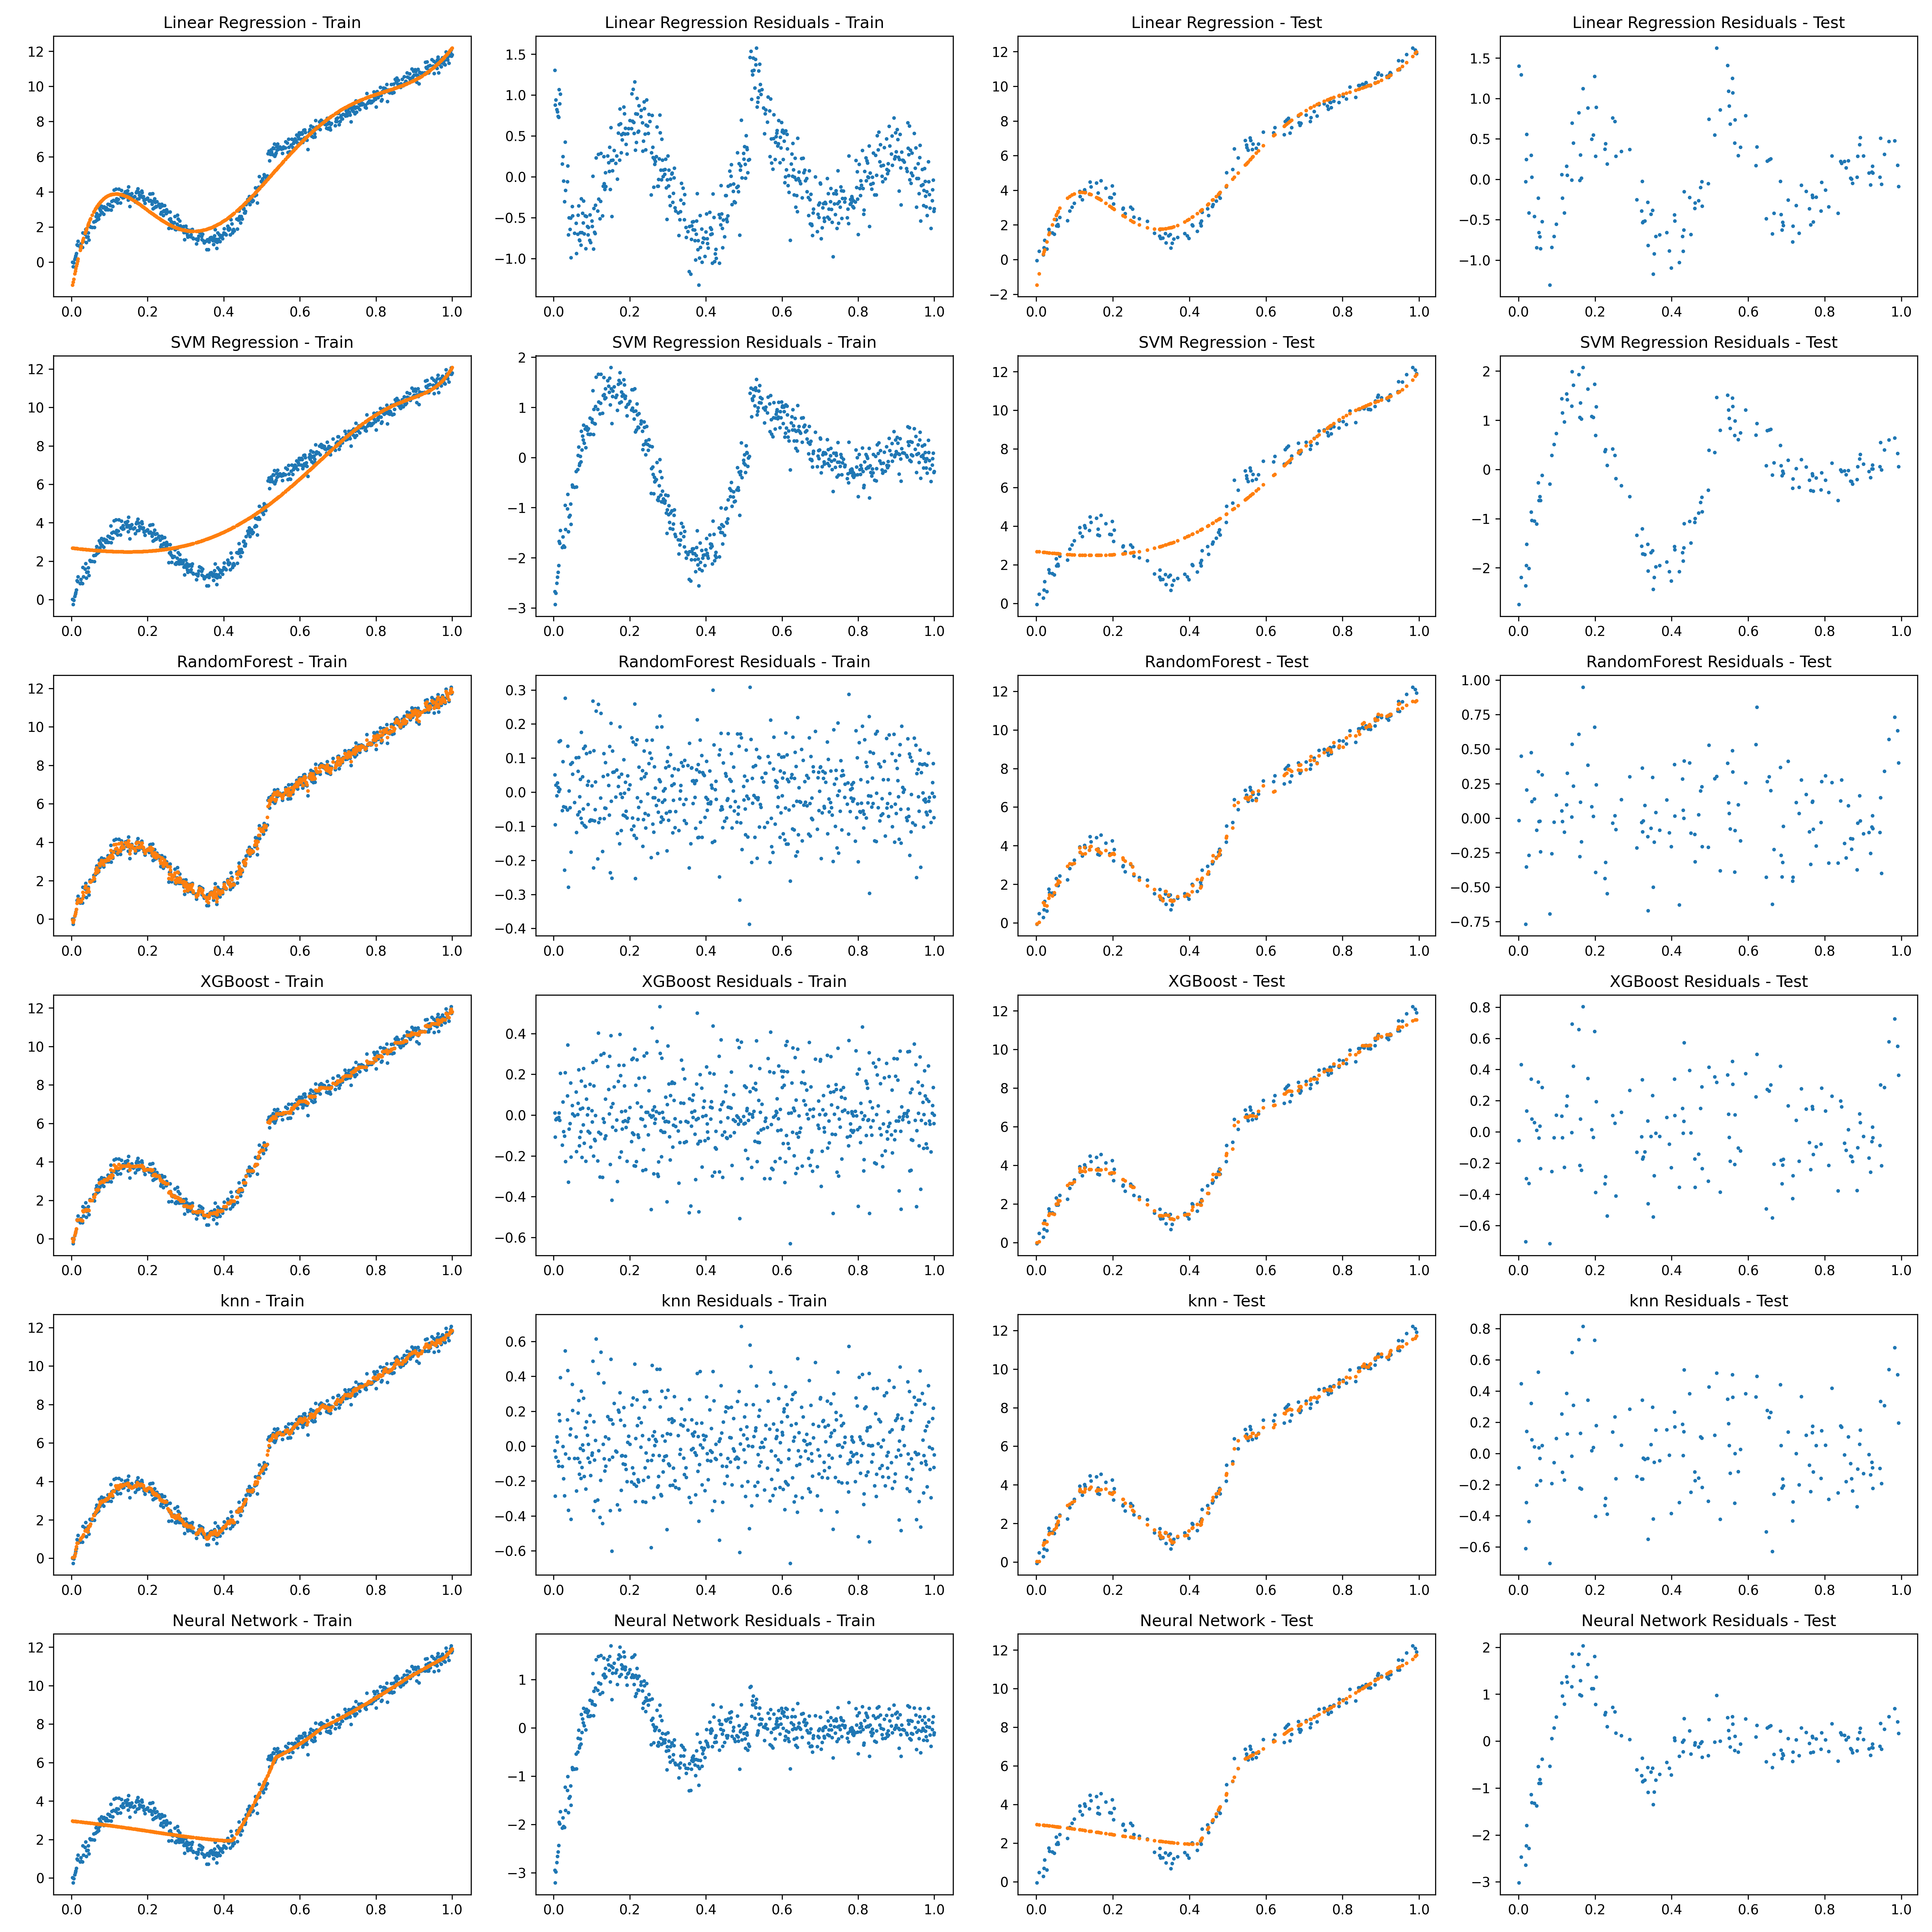
\includegraphics[width=0.8\linewidth]{./Images/E3-MLR3-6.png}
	\caption{Various Regression Models with degree = 6}
\end{figure}

\begin{itemize}
    \item \textbf{Linear Regression:} The plot shows significant overfitting, with the linear model failing to generalize and fitting the noise in the data rather than the true underlying pattern.
    \item \textbf{SVM (Polynomial Kernel):} The linear SVM plot still exhibits overfitting, with the decision boundary overly complex and not effectively capturing the true non-linear structure of the data.
    \item \textbf{RandomForest:} The plot demonstrates excellent fit to the data, capturing the intricate non-linear patterns, though it may start to show signs of overfitting with the increased feature complexity.
    \item \textbf{XGBoost:} The XGBoost plot reveals strong performance, modeling complex non-linear relationships well, but may also show signs of overfitting as the model captures noise along with the signal.
    \item \textbf{K-Nearest Neighbors (KNN):} The KNN plot shows a good fit, accurately following the non-linear data trends; however, it may become sensitive to noise with the increased feature space.
    \item \textbf{Neural Network:} The Neural Network plot indicates an excellent fit to the data, effectively capturing complex non-linear patterns with the expanded feature set, though it may also exhibit overfitting.
\end{itemize}

\begin{figure}[H]
	\centering
	\includegraphics[width=0.8\linewidth]{./Images/E3-MLR3-10.png}
	\caption{Various Regression Models with degree = 10}
\end{figure}

\begin{itemize}
    \item \textbf{Linear Regression:} The plot shows severe overfitting, with the linear model failing to generalize and fitting the data's noise, resulting in a very erratic fit that does not align well with the true underlying patterns.
    \item \textbf{SVM (Polynomial Kernel):} The linear SVM plot also displays significant overfitting, with the decision boundary becoming overly complex and not effectively capturing the non-linear data structure.
    \item \textbf{RandomForest:} The plot demonstrates a very good fit to the complex data, but signs of overfitting are evident, as the model captures both the noise and the intricate non-linear patterns.
    \item \textbf{XGBoost:} The XGBoost plot shows exceptional fit, accurately capturing the complex non-linear relationships; however, overfitting is pronounced, with the model fitting noise along with the data signal.
    \item \textbf{K-Nearest Neighbors (KNN):} The KNN plot shows an excellent fit, with predictions following the non-linear trends closely; however, the model is highly sensitive to noise due to the high dimensionality.
    \item \textbf{Neural Network:} The Neural Network plot reveals a strong fit to the data, capturing intricate non-linear patterns effectively; overfitting is apparent as the model fits the noise in addition to the data signal.
\end{itemize}

\clearpage

\begin{customboxnew}[label={box:Q3b}]{Question (b)}
	Create an overall qualitative summary based on a review and analysis of the Figures generated.
\end{customboxnew}

The analysis of the figures for training and testing data, as well as the corresponding errors, across different models and polynomial degrees provides insights into how well each model handles the increasing complexity introduced by polynomial feature expansion.

\begin{itemize}
    \item \textbf{Degree = 1:}
    \begin{itemize}
        \item \textbf{Training Data:} The plots show that all models, except for non-parametric methods (KNN and Neural Networks), fail to capture the non-linear patterns present in the data. Linear Regression and SVM with a polynomial kernel exhibit a clear inability to fit the data, resulting in large discrepancies between predicted and true values.
        \item \textbf{Error in Training Data:} Errors are relatively high for Linear Regression and linear SVM, reflecting poor fit. RandomForest, XGBoost, KNN, and Neural Networks show lower training errors, as they can model non-linear patterns better without polynomial feature expansion.
        \item \textbf{Testing Data:} Similar patterns are observed in testing data plots, where models assuming linear relationships (Linear Regression and linear SVM) perform poorly. RandomForest, XGBoost, KNN, and Neural Networks perform better by capturing the underlying non-linearities.
        \item \textbf{Error in Testing Data:} The errors for Linear Regression and linear SVM are high, while RandomForest, XGBoost, KNN, and Neural Networks show lower testing errors, indicating better generalization to unseen data.
    \end{itemize}

    \item \textbf{Degree = 3:}
    \begin{itemize}
        \item \textbf{Training Data:} The addition of polynomial terms up to degree 3 improves the fit for Linear Regression and linear SVM, with plots showing a closer alignment to the data. Non-parametric methods like RandomForest, XGBoost, KNN, and Neural Networks continue to perform well.
        \item \textbf{Error in Training Data:} Training errors for Linear Regression and linear SVM decrease as polynomial features help capture more of the non-linear structure. RandomForest and XGBoost maintain low errors, while KNN and Neural Networks exhibit consistent performance.
        \item \textbf{Testing Data:} The improvement in fit is also seen in testing data plots, with Linear Regression and linear SVM showing better generalization. Non-parametric models maintain strong performance with reduced testing errors.
        \item \textbf{Error in Testing Data:} Testing errors decrease for Linear Regression and linear SVM due to better fit with polynomial features. Non-parametric models continue to show low errors, indicating robust performance.
    \end{itemize}

    \item \textbf{Degree = 6:}
    \begin{itemize}
        \item \textbf{Training Data:} With polynomial terms up to degree 6, Linear Regression and linear SVM fit the training data very closely, showing complex curves that align well with the data. Non-parametric models still capture the non-linear patterns effectively.
        \item \textbf{Error in Training Data:} Training errors for all models decrease, with Linear Regression and linear SVM potentially showing very low errors, indicating overfitting. Non-parametric models continue to perform well with low training errors.
        \item \textbf{Testing Data:} The fit on testing data shows that models may start overfitting, with complex curves in Linear Regression and linear SVM potentially fitting the noise rather than the true pattern. Non-parametric methods manage the complexity better.
        \item \textbf{Error in Testing Data:} Testing errors for Linear Regression and linear SVM might increase due to overfitting, while non-parametric models maintain relatively low errors.
    \end{itemize}

    \item \textbf{Degree = 10:}
    \begin{itemize}
        \item \textbf{Training Data:} The fit for degree 10 features shows significant overfitting for Linear Regression and linear SVM, with highly complex curves that fit the training data extremely well but may not generalize. Non-parametric models handle the complexity more gracefully.
        \item \textbf{Error in Training Data:} Training errors are very low for Linear Regression and linear SVM due to overfitting, whereas non-parametric models still show low errors but with potential signs of overfitting.
        \item \textbf{Testing Data:} Testing data plots reveal poor generalization for Linear Regression and linear SVM, with predictions diverging from true values due to overfitting. Non-parametric methods generally continue to show better performance.
        \item \textbf{Error in Testing Data:} Testing errors are high for Linear Regression and linear SVM due to overfitting, while non-parametric methods exhibit moderate errors, showing better generalization to unseen data.
    \end{itemize}
\end{itemize}

\begin{customboxnew}[label={box:Q3c}]{Question (c)}
	Summarize and explain the variations in the metrics \textbf{across regression methods for a given degree} (ie. a given set of polynomial features). Cover both, train and test, metrics, and compare them.
\end{customboxnew}

For each polynomial degree, the following analysis compares the performance of different regression methods based on their training and testing metrics.

\subsubsection*{Degree = 1}

\begin{figure}[H]
    \centering
    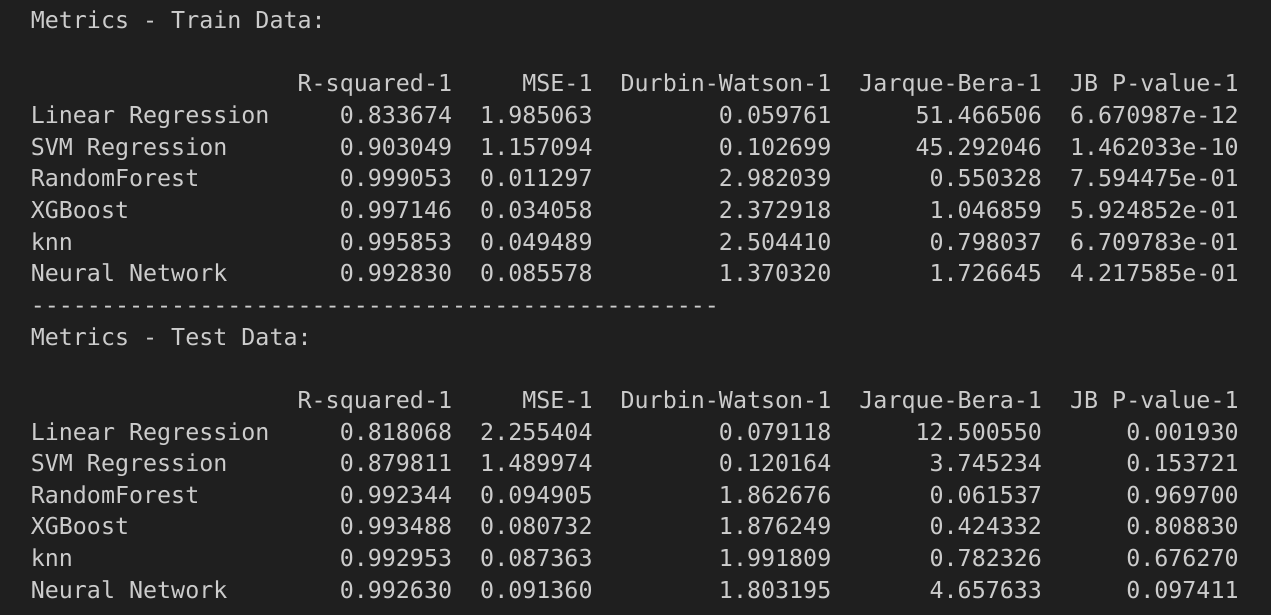
\includegraphics[width=0.8\linewidth]{./Images/Error-Metrics-Degree-1.png}
    \caption{Various Regression Models with degree = 1}
\end{figure}

At \textbf{degree = 1}, with only linear features:

\begin{itemize}
    \item \textbf{Linear Regression and SVM (Linear Kernel):} 
    \begin{itemize}
        \item \textbf{Training and Testing Metrics:} High, as these models cannot capture non-linear relationships effectively.
    \end{itemize}
    
    \item \textbf{RandomForest, XGBoost, KNN, Neural Network:}
    \begin{itemize}
        \item \textbf{Training and Testing Metrics:} Low, showing strong performance and good generalization even with linear features.
    \end{itemize}
\end{itemize}

\subsubsection*{Degree = 3}

\begin{figure}[H]
    \centering
    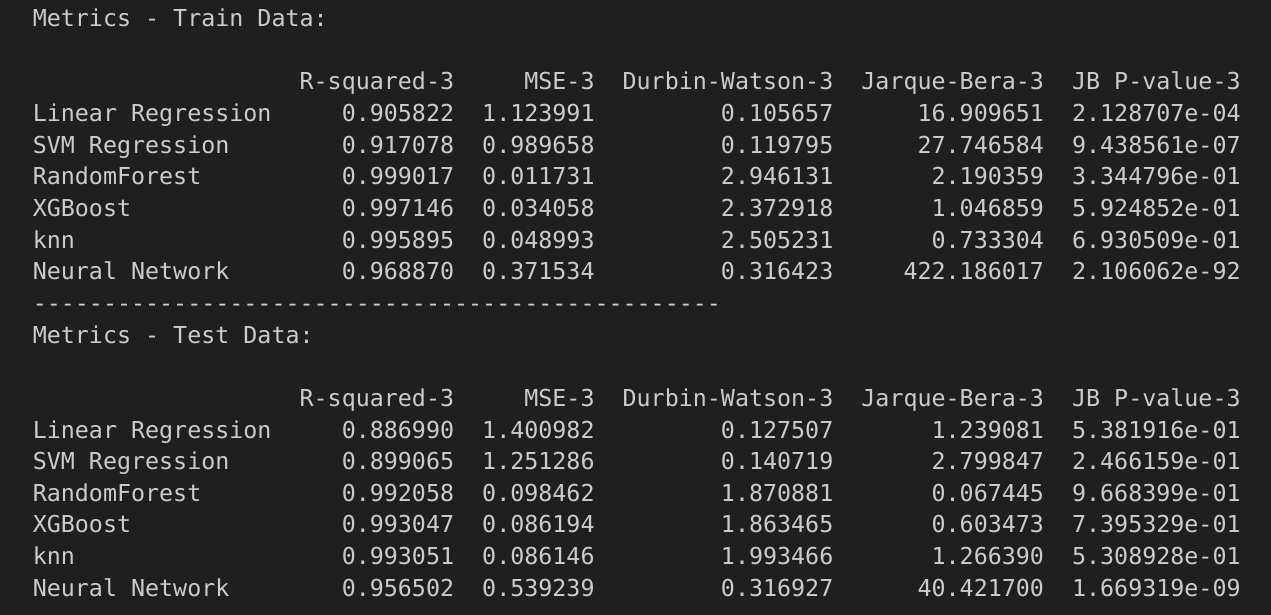
\includegraphics[width=0.8\linewidth]{./Images/Error-Metrics-Degree-3.png}
    \caption{Various Regression Models with degree = 3}
\end{figure}

At \textbf{degree = 3}, with cubic features:

\begin{itemize}
    \item \textbf{Linear Regression and SVM (Linear Kernel):} 
    \begin{itemize}
        \item \textbf{Training and Testing Metrics:} Improved, capturing more non-linear patterns compared to degree 1, though still limited.
    \end{itemize}
    
    \item \textbf{RandomForest, XGBoost, KNN, Neural Network:}
    \begin{itemize}
        \item \textbf{Training and Testing Metrics:} Remain low, reflecting effective use of cubic features and continued strong performance.
    \end{itemize}
\end{itemize}

\subsubsection*{Degree = 6}

\begin{figure}[H]
    \centering
    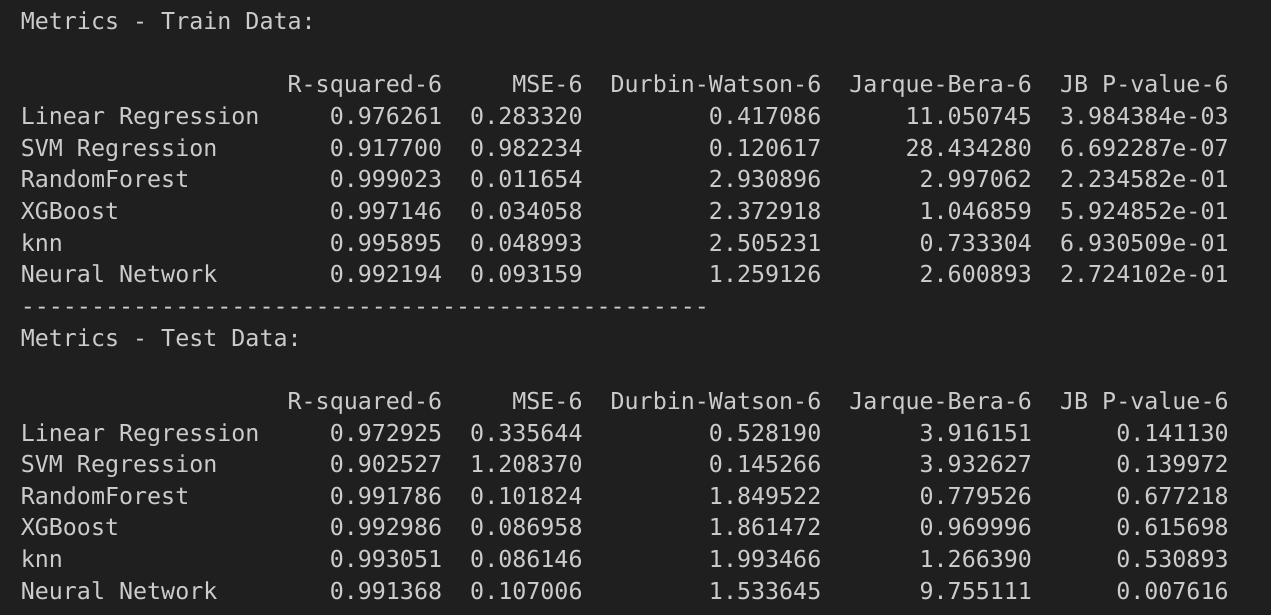
\includegraphics[width=0.8\linewidth]{./Images/Error-Metrics-Degree-6.png}
    \caption{Various Regression Models with degree = 6}
\end{figure}

At \textbf{degree = 6}, with higher polynomial features:

\begin{itemize}
    \item \textbf{Linear Regression and SVM (Linear Kernel):} 
    \begin{itemize}
        \item \textbf{Training Metrics:} Significantly improved, fitting the data better. Testing metrics may start to increase due to overfitting.
    \end{itemize}
    
    \item \textbf{RandomForest, XGBoost, KNN, Neural Network:}
    \begin{itemize}
        \item \textbf{Training Metrics:} Very low, capturing complex patterns. Testing metrics may rise slightly due to potential overfitting.
    \end{itemize}
\end{itemize}

\subsubsection*{Degree = 10}

\begin{figure}[H]
    \centering
    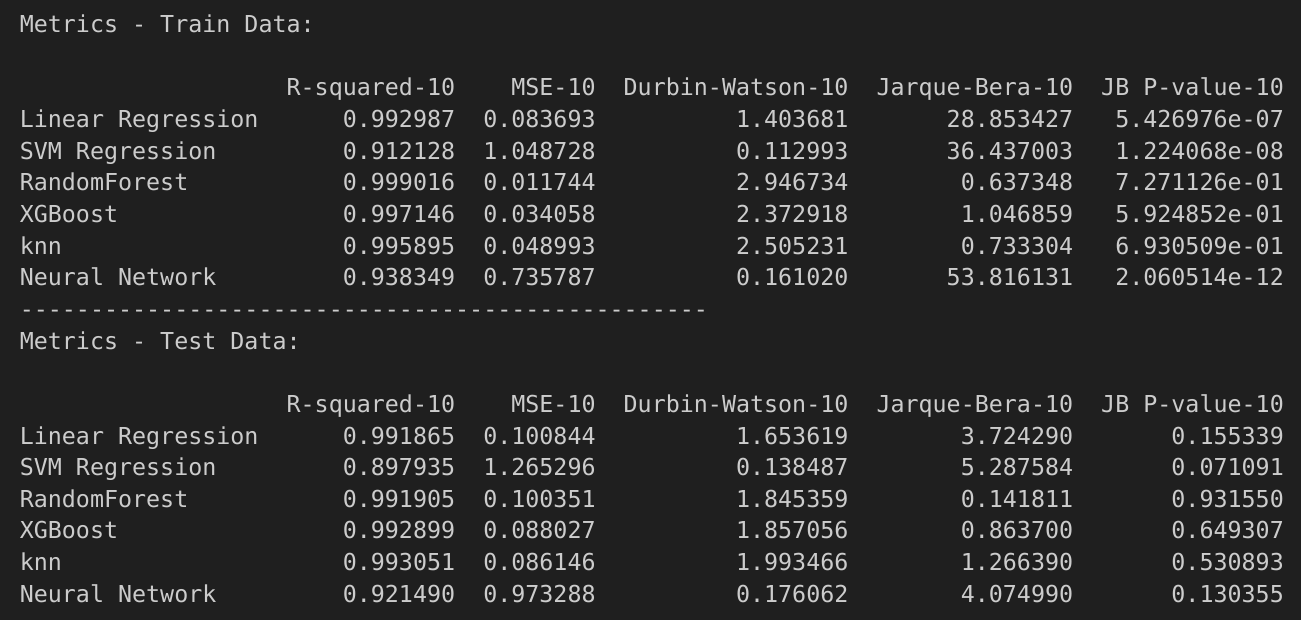
\includegraphics[width=0.8\linewidth]{./Images/Error-Metrics-Degree-10.png}
    \caption{Various Regression Models with degree = 10}
\end{figure}

At \textbf{degree = 10}, with even more complex features:

\begin{itemize}
    \item \textbf{Linear Regression and SVM (Linear Kernel):} 
    \begin{itemize}
        \item \textbf{Training Metrics:} Extremely low due to overfitting. Testing metrics often increase significantly, reflecting poor generalization.
    \end{itemize}
    
    \item \textbf{RandomForest, XGBoost, KNN, Neural Network:}
    \begin{itemize}
        \item \textbf{Training Metrics:} Very low, but testing metrics typically rise, showing overfitting and decreased generalization.
    \end{itemize}
\end{itemize}

In summary, as polynomial degree increases, models that are inherently prone to overfitting (such as Linear Regression and polynomial SVM) show severe overfitting with very low training errors but higher testing errors. Non-parametric methods (RandomForest, XGBoost, KNN, Neural Networks) tend to handle increased feature complexity better, but may also exhibit signs of overfitting as the degree of the polynomial features increases. The performance of each model highlights the trade-off between fitting complex patterns in training data and generalizing to unseen data.

\clearpage

\begin{customboxnew}[label={box:Q3d}]{Question (d)}
	Summarize and explain the variations in the metrics \textbf{across degrees for a given regression method}. Cover both, train, and test metrics, and compare them.
\end{customboxnew}

\subsubsection*{Linear Regression}

\begin{itemize}
    \item \textbf{Degree = 1:} High training and testing metrics, poor fit.
    \item \textbf{Degree = 3:} Improved metrics, better fit but still limited.
    \item \textbf{Degree = 6:} Very low training metrics, higher testing metrics due to overfitting.
    \item \textbf{Degree = 10:} Extremely low training metrics, high testing metrics indicating severe overfitting.
\end{itemize}

\subsubsection*{SVM (Polynomial Kernel)}

\begin{itemize}
    \item \textbf{Degree = 1:} High metrics, inadequate for non-linear data.
    \item \textbf{Degree = 3:} Lower metrics, better fit for non-linearities.
    \item \textbf{Degree = 6:} Low metrics, may overfit.
    \item \textbf{Degree = 10:} Very low training metrics, high testing metrics due to overfitting.
\end{itemize}

\subsubsection*{RandomForest, XGBoost, KNN, Neural Network}

\begin{itemize}
    \item \textbf{Degree = 1:} Low metrics, good fit even with linear features.
    \item \textbf{Degree = 3:} Low metrics, enhanced by cubic features.
    \item \textbf{Degree = 6:} Very low metrics, potential for slight overfitting.
    \item \textbf{Degree = 10:} Extremely low training metrics, higher testing metrics due to overfitting.
\end{itemize}

% \clearpage

\begin{customboxnew}[label={box:Q3e}]{Question (e)}
	When \textbf{degree = 1} which method(s) result in acceptable regression models? Why?
\end{customboxnew}

When \textbf{degree = 1}, the following methods result in acceptable regression models:

\begin{itemize}
    \item \textbf{RandomForest, XGBoost, KNN, Neural Network:} Provide acceptable performance with low training and testing metrics, as they can handle non-linear relationships effectively even with linear features.
    \item \textbf{Linear Regression, SVM (Linear Kernel):} Typically result in poor models with high training and testing metrics, due to their inability to capture non-linear patterns.
\end{itemize}

\begin{customboxnew}[label={box:Q3f}]{Question (f)}
	When \textbf{degree = 6} which method(s) result in acceptable regression models? Why?
\end{customboxnew}

When \textbf{degree = 6}, the following methods result in acceptable regression models:

\begin{itemize}
    \item \textbf{RandomForest, XGBoost, KNN, Neural Network:} Handle the complexity of polynomial features well, providing low training metrics and acceptable testing metrics, despite some potential for overfitting.
    \item \textbf{Linear Regression, SVM (Polynomial Kernel):} May exhibit good training performance but often have high testing metrics due to overfitting with higher polynomial degrees.
\end{itemize}

\clearpage

\begin{customboxnew}[label={box:Q3g}]{Question (g)}
	As the value of degree is increased to 10 which regression methods show the most impact? Why?
\end{customboxnew}

As the polynomial degree increases to \textbf{10}, the following methods show the most impact:

\begin{itemize}
    \item \textbf{Linear Regression, SVM (Polynomial Kernel):} Experience significant overfitting, resulting in extremely low training metrics and high testing metrics, reflecting poor generalization.
    \item \textbf{RandomForest, XGBoost, KNN, Neural Network:} Also show overfitting with very low training metrics and higher testing metrics, though they manage complexity better than linear models.
\end{itemize}

\begin{customboxnew}[label={box:Q3h}]{Question (h)}
	Why do non-parametric methods like \verb|KNN| and \verb|Decision Tree| based methods generate good results even without feature engineering?
\end{customboxnew}

Non-parametric methods like \texttt{KNN} and \texttt{Decision Tree} generate good results even without feature engineering because:

\begin{itemize}
    \item \textbf{KNN (K-Nearest Neighbors):} Relies on local similarity, capturing complex patterns directly from the data without needing explicit feature transformations.
    \item \textbf{Decision Trees:} Automatically learn interactions and hierarchies in data through splits, adapting to various patterns without requiring pre-engineered features.
\end{itemize}

% \clearpage

\begin{customboxnew}[label={box:Q3i}]{Question (i)}
	What are the limitations of the non-parametric methods?
\end{customboxnew}

Non-parametric methods like \texttt{KNN} and \texttt{Decision Tree} have the following limitations:

\begin{itemize}
    \item \textbf{KNN (K-Nearest Neighbors):}
    \begin{itemize}
        \item \textbf{Computational Complexity:} Slow prediction times as it requires calculating distances to all training samples.
        \item \textbf{Curse of Dimensionality:} Performance degrades with high-dimensional data, as distance metrics become less meaningful.
    \end{itemize}
    
    \item \textbf{Decision Trees:}
    \begin{itemize}
        \item \textbf{Overfitting:} Can easily overfit the training data, especially with deep trees.
        \item \textbf{Instability:} Small changes in data can lead to different tree structures, making them sensitive to noise.
    \end{itemize}
\end{itemize}

\begin{customboxnew}[label={box:Q3j}]{Question (j)}
	Given the results, should \verb|LinearRegression| be used at all? Why, when? Justify your answer.
\end{customboxnew}

Given the results, \verb|LinearRegression| should be used in the following contexts:

\begin{itemize}
    \item \textbf{When Data is Linearly Correlated:} Linear Regression is effective when the relationship between features and target variable is approximately linear.
    \item \textbf{For Simplicity and Interpretability:} It offers simplicity and easy interpretation of coefficients, making it useful for quick insights and when model interpretability is crucial.
    \item \textbf{When Overfitting is a Concern:} It can serve as a baseline model or when you want to avoid the complexity and overfitting risks associated with more flexible models.
\end{itemize}

However, for non-linear relationships or when higher degrees of complexity are needed, more advanced methods like RandomForest, XGBoost, or Neural Networks may be preferred.

% \clearpage

\section*{Error Metrics}

\begin{figure}[H]
    \centering
    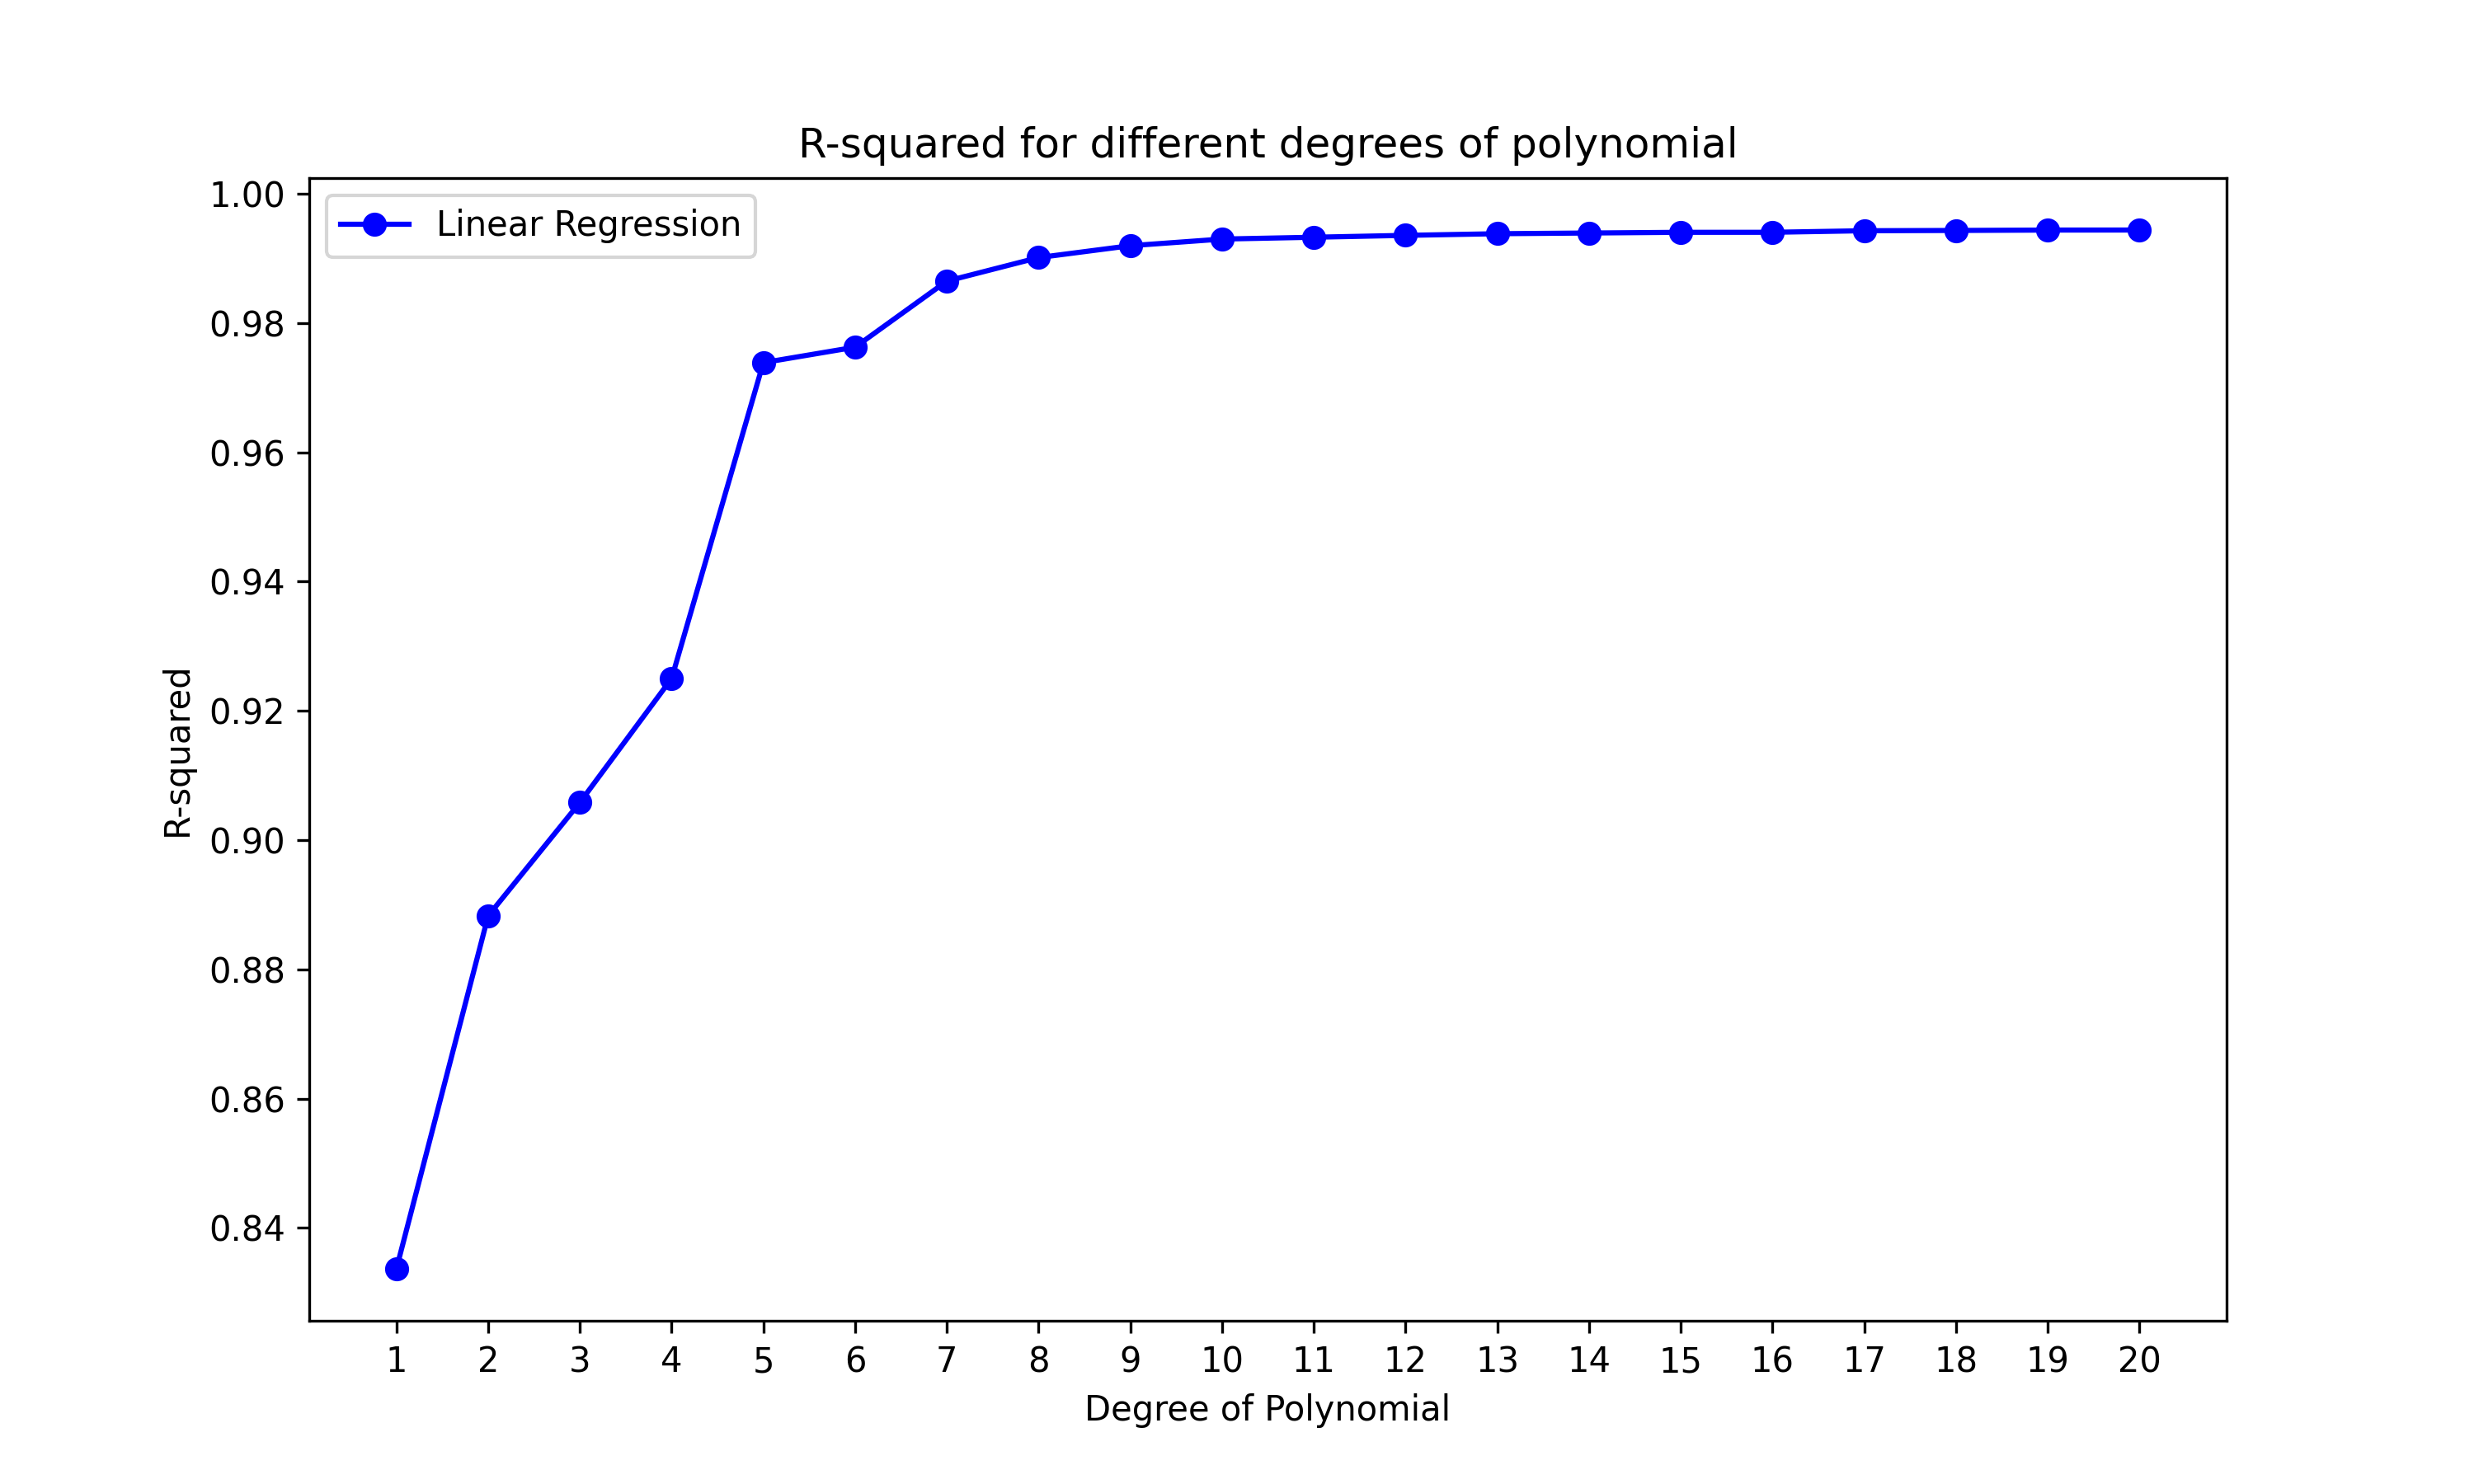
\includegraphics[width=0.5\linewidth]{./Images/R-squared.png}
    \caption{R-squared Error Metric}
\end{figure}

\begin{figure}[H]
    \centering
    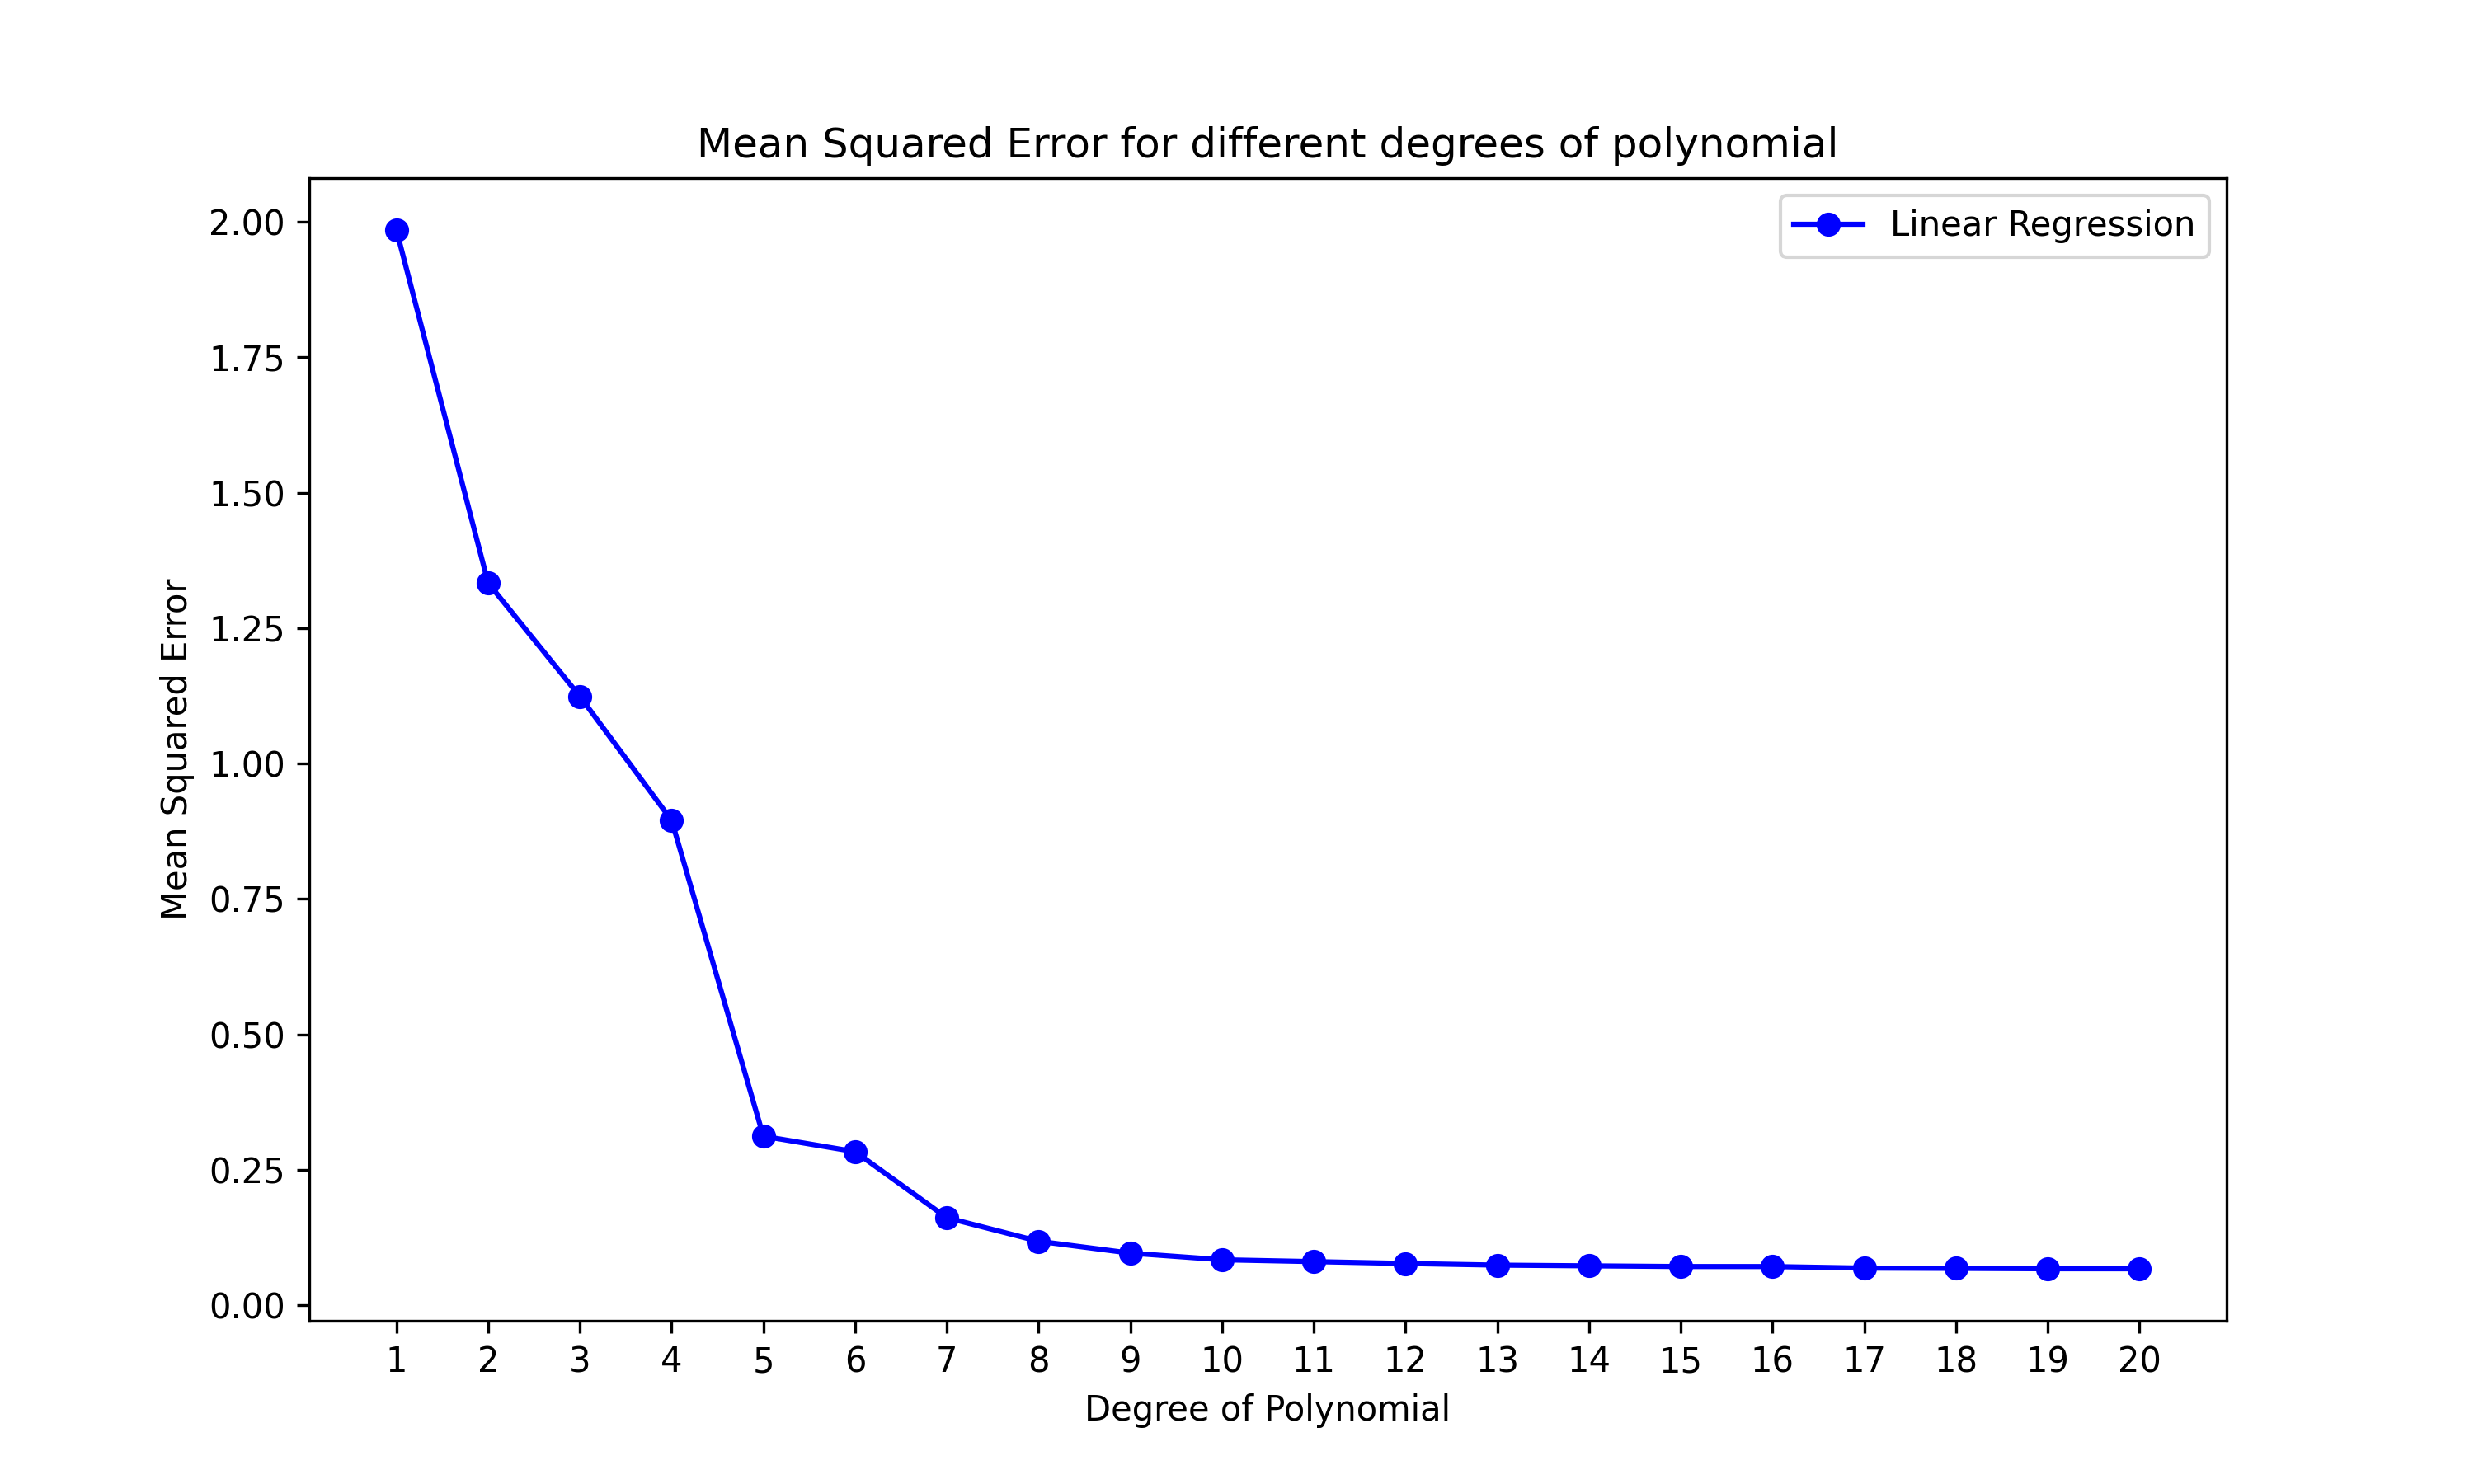
\includegraphics[width=0.5\linewidth]{./Images/MSE.png}
    \caption{Mean Squared Error Metric}
\end{figure}

\begin{figure}[H]
    \centering
    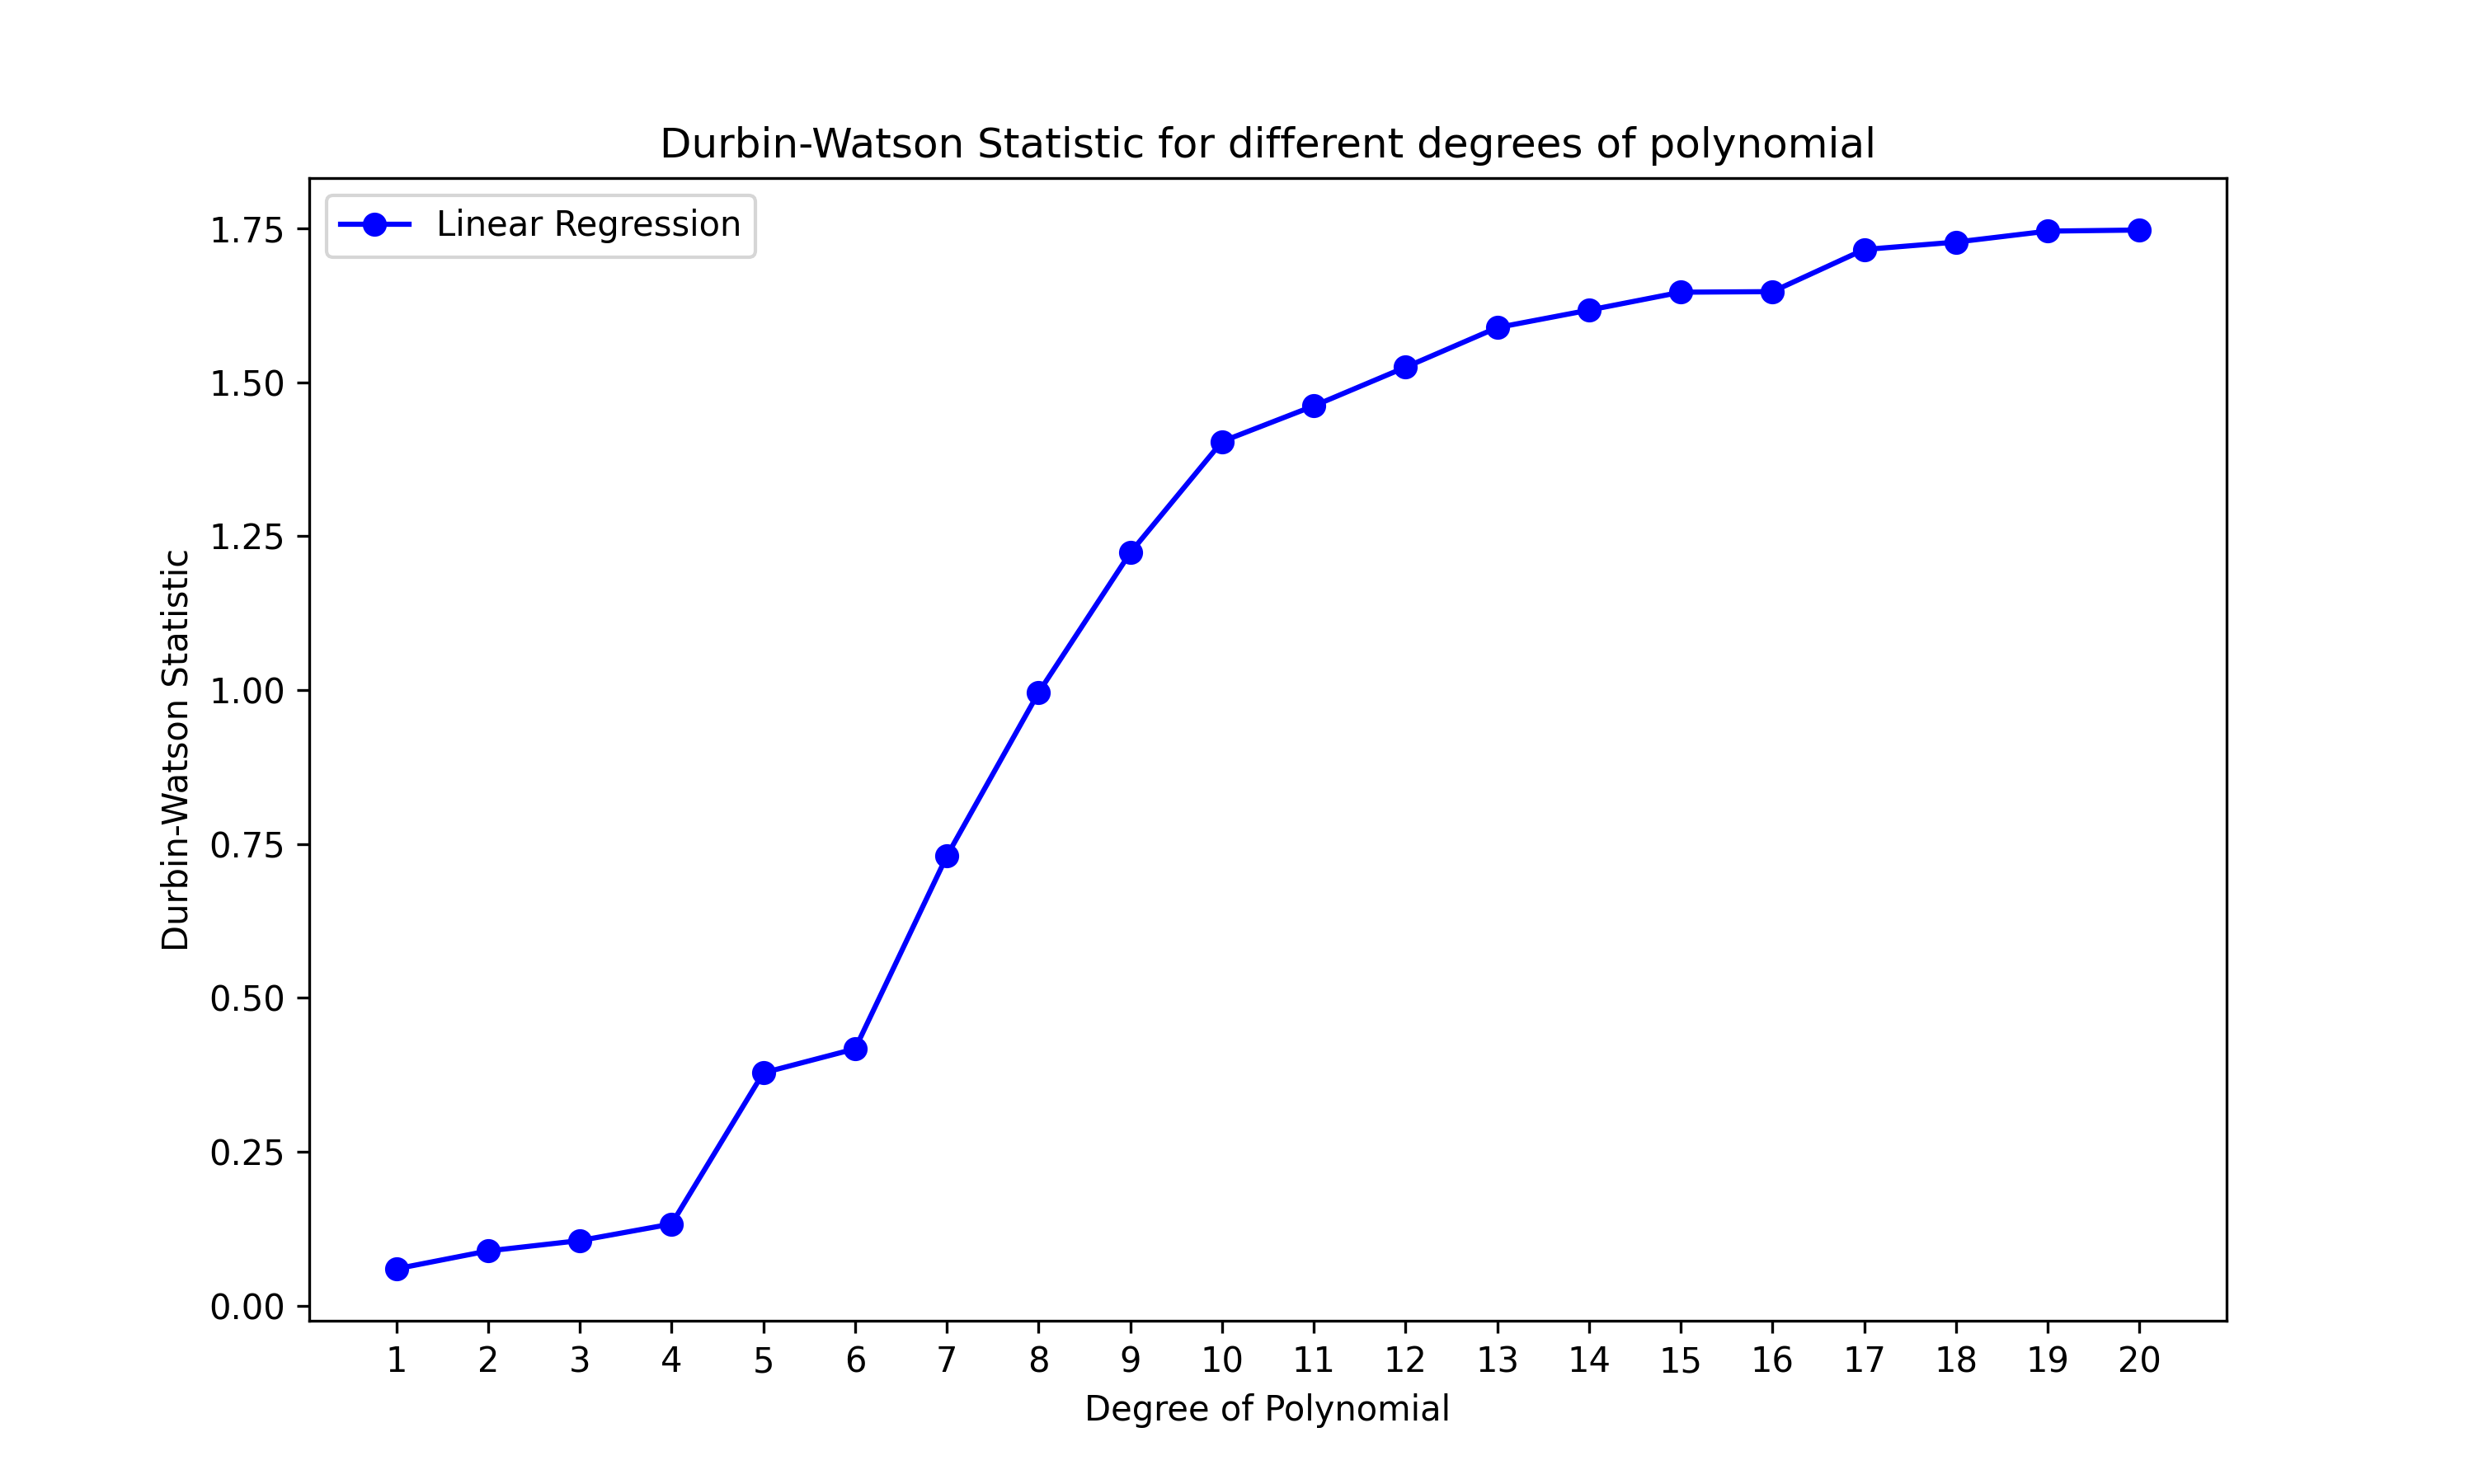
\includegraphics[width=0.5\linewidth]{./Images/Durbin-Watson.png}
    \caption{Durbin-Watson Error Metric}
\end{figure}

\begin{figure}[H]
    \centering
    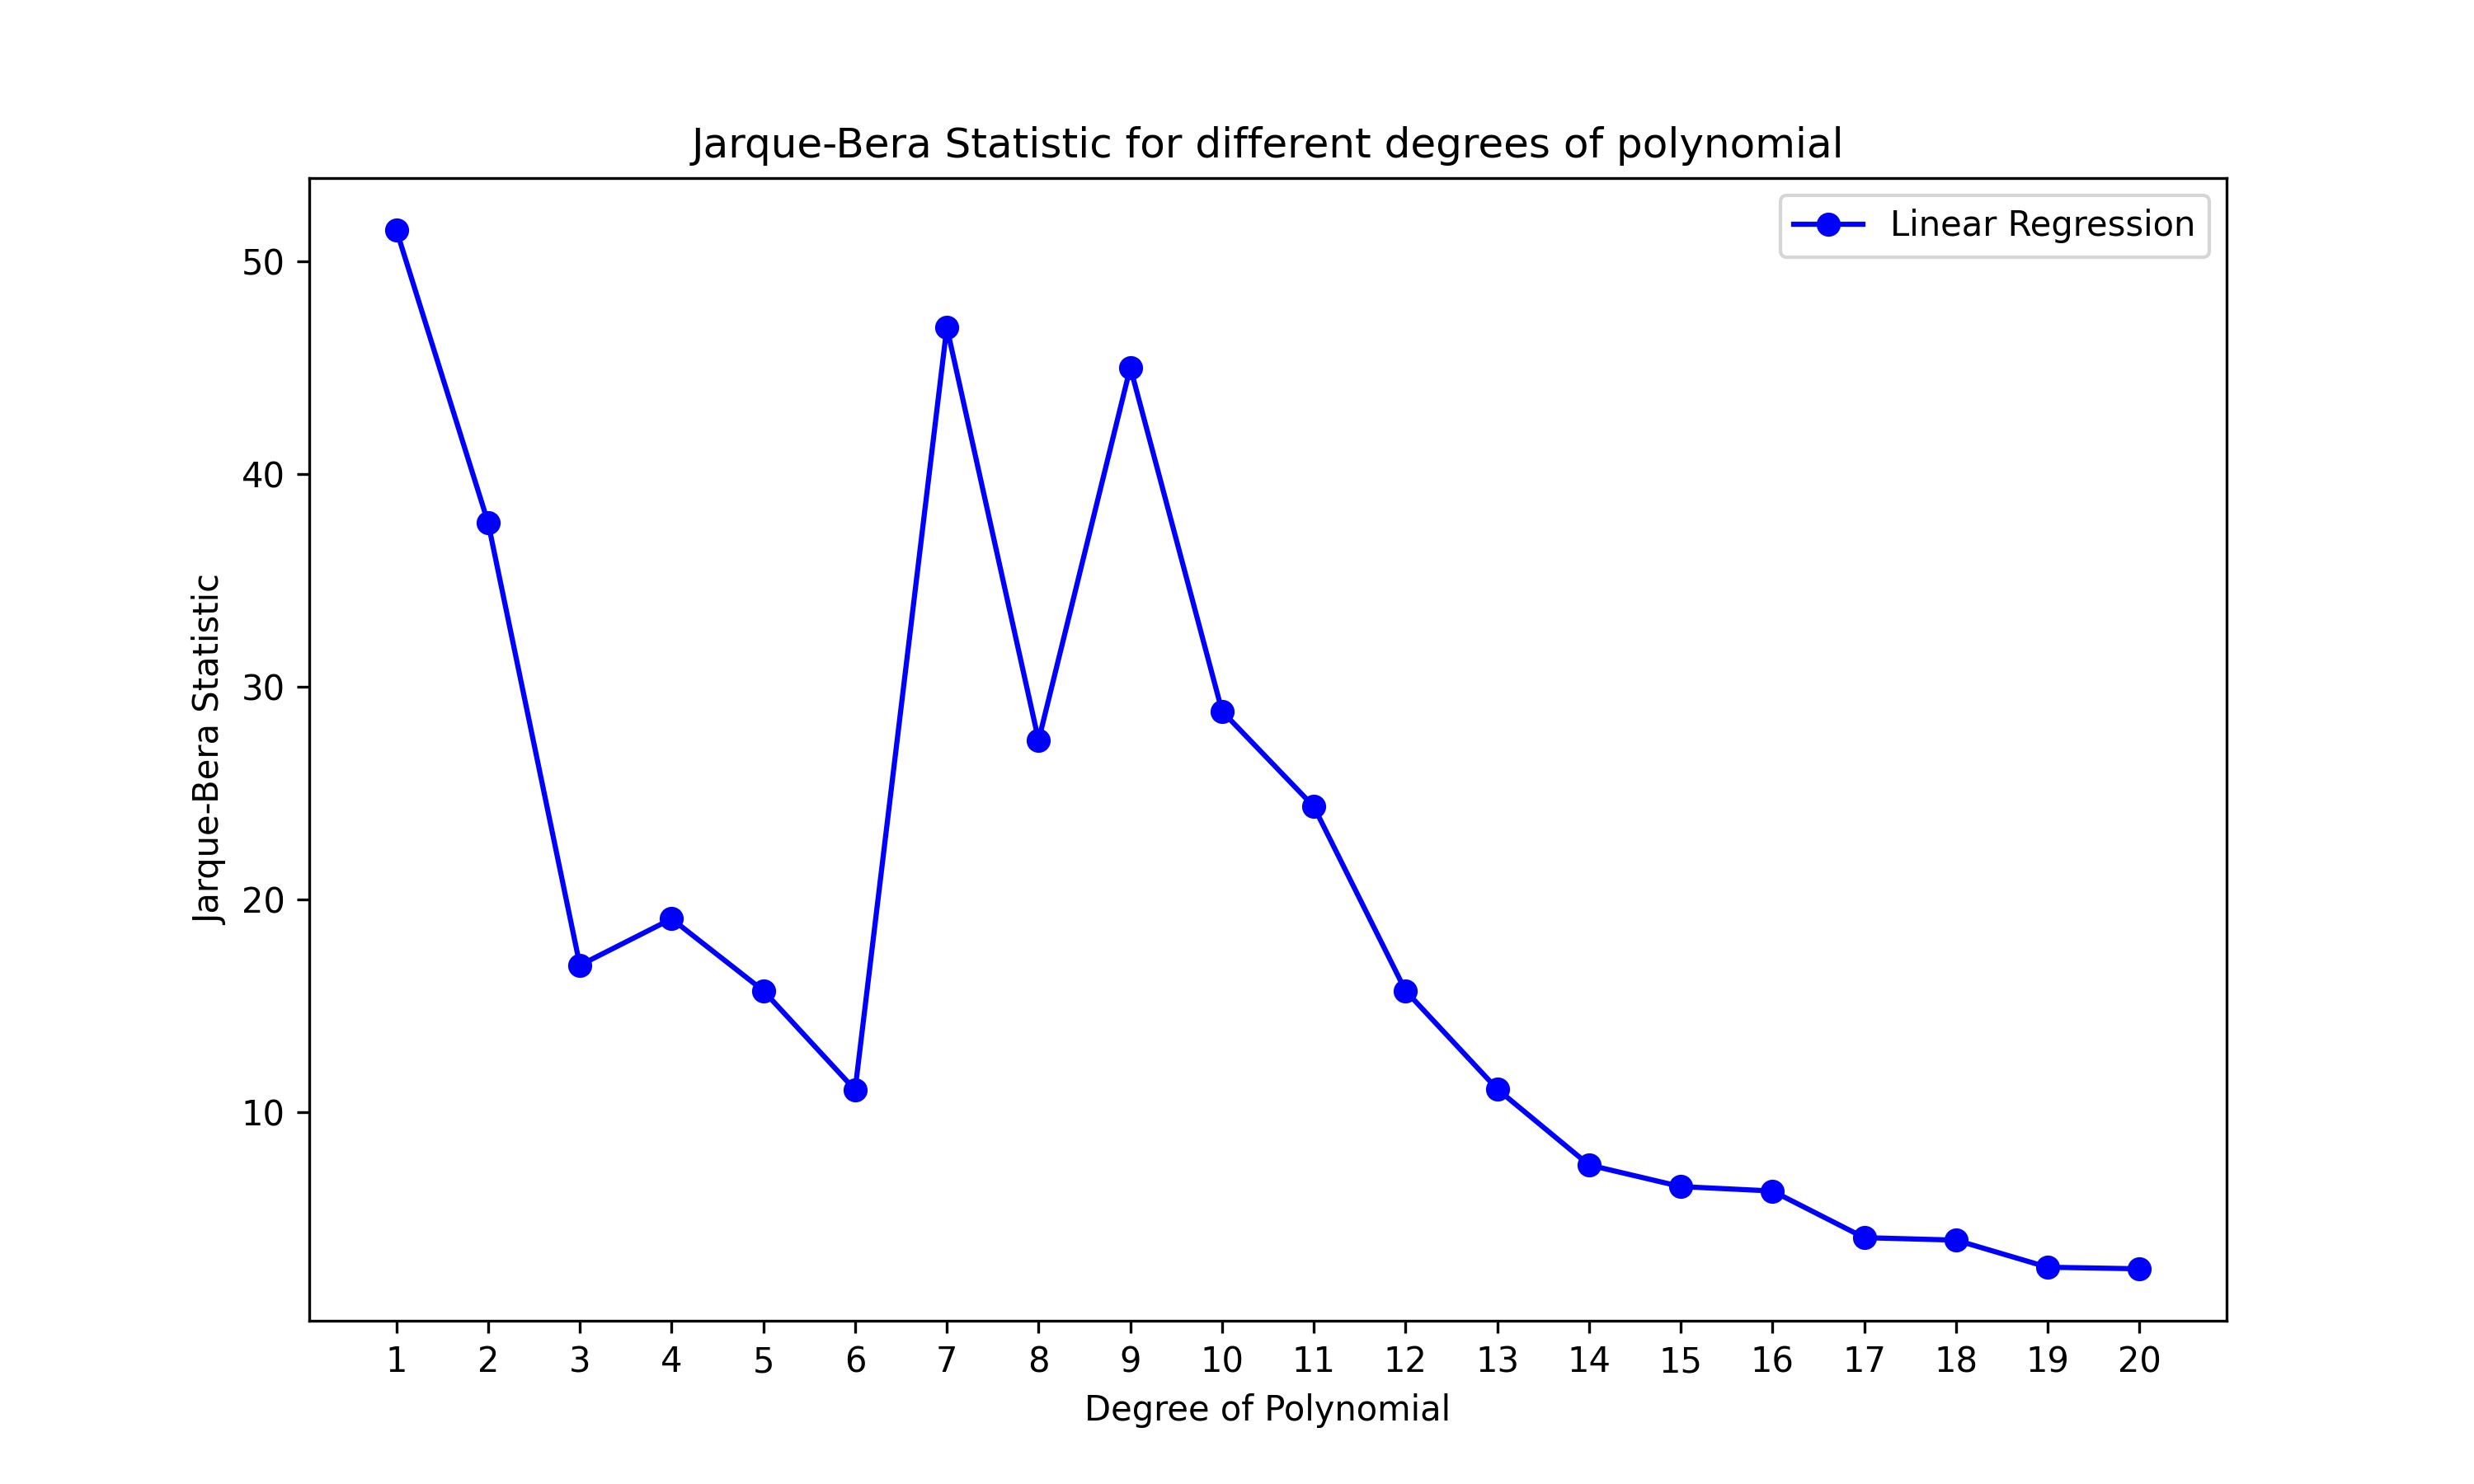
\includegraphics[width=0.5\linewidth]{./Images/Jarque-Bera.png}
    \caption{Jarque-Bera Error Metric}
\end{figure}

\begin{figure}[H]
    \centering
    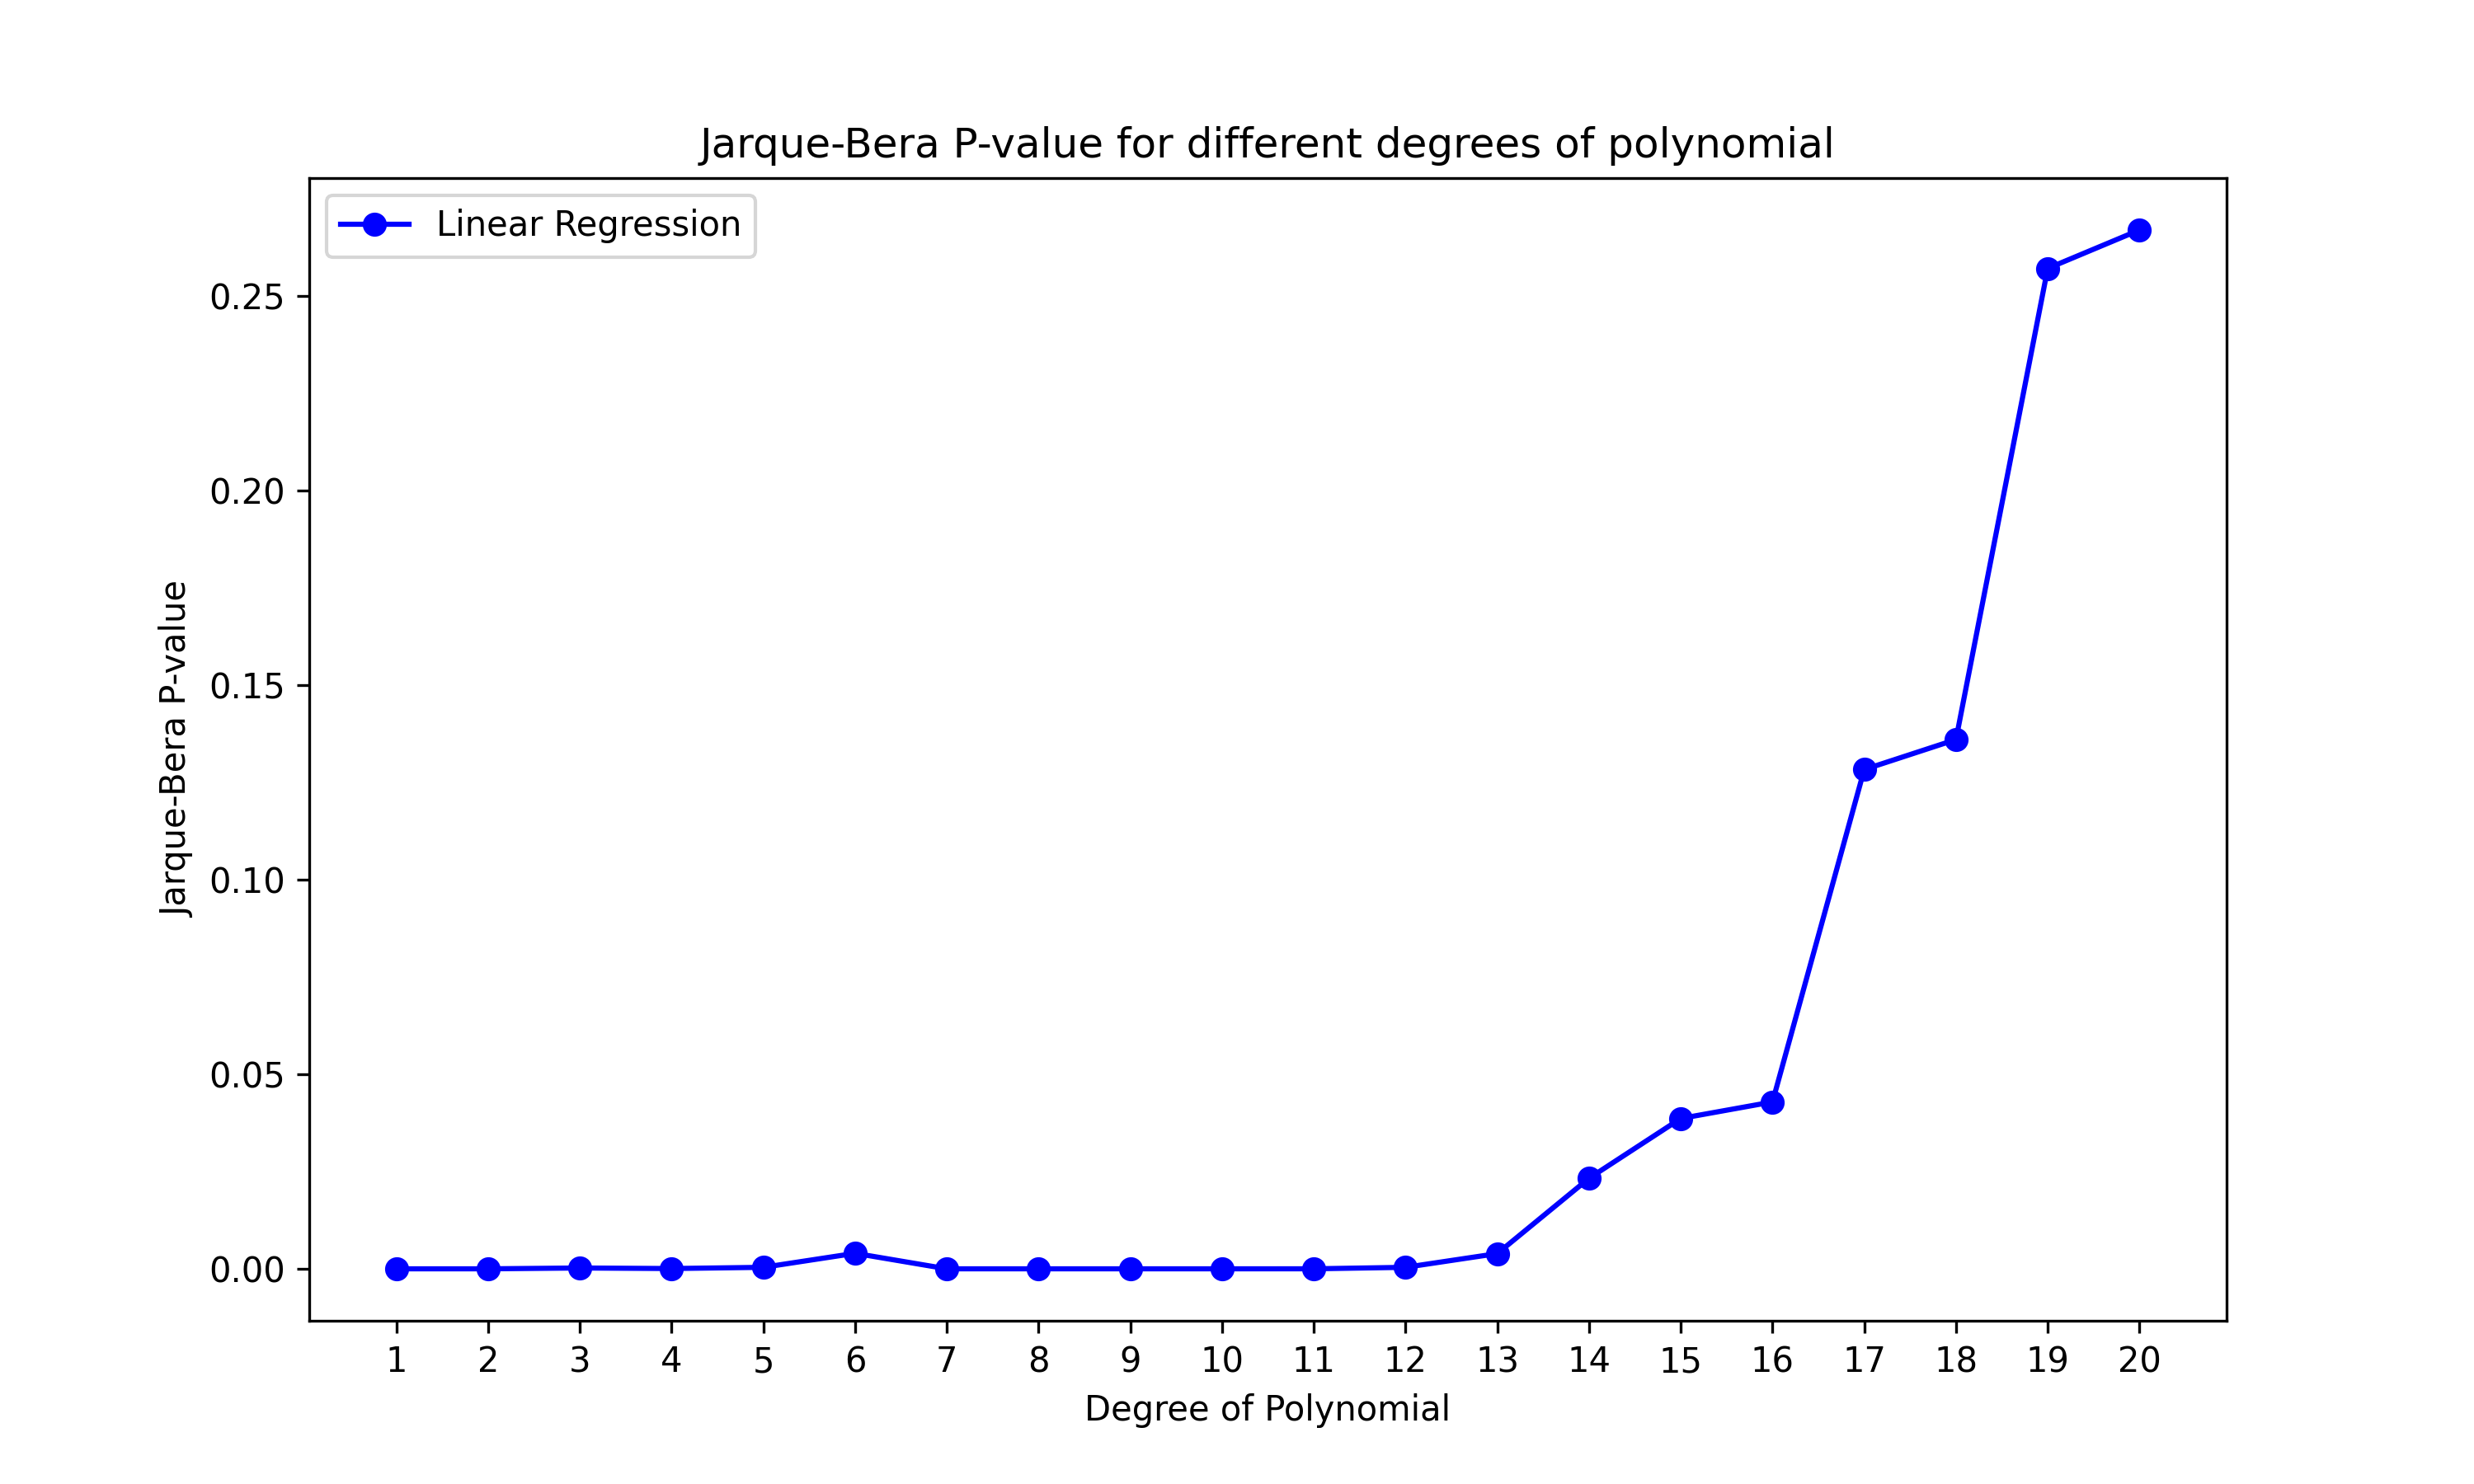
\includegraphics[width=0.5\linewidth]{./Images/JB-P-value.png}
    \caption{Jarque-Bera P-value Error Metric}
\end{figure}

We observe that the error metrics provide insights into the model's performance, with R-squared indicating the proportion of variance explained, MSE quantifying prediction errors, Durbin-Watson testing for autocorrelation, and Jarque-Bera assessing normality. These metrics help evaluate the model's fit, generalization, and assumptions, guiding model selection and interpretation.

\begin{enumerate}[label=(\alph*)]
    \item \textbf{R-squared:} The $R^2$ metric for degree from $1$ to $20$ shows an increasing trend as degree of the polynomial features increases. 
    \item \textbf{Mean Squared Error (MSE):} The MSE decreases with increasing degree, indicating better model fit and lower prediction errors.
    \item \textbf{Durbin-Watson:} The Durbin-Watson statistic is increasingly close to $2$ for higher degrees, suggesting reduced autocorrelation in the residuals.
    \item \textbf{Jarque-Bera:} The Jarque-Bera statistic and its p-value show deviations from normality, with higher degrees exhibiting more significant deviations.
\end{enumerate}

\clearpage